\section{Base Teórica}\label{sec:base}

\subsection{Métricas de Erros}\label{subsec:metrica}

A métrica MSE é uma das mais utilizadas em aprendizado de máquina. Seu cálculo é feito da seguinte forma:

\begin{eqnarray}
	M S E=\dfrac{1}{n} \sum\left(y_i-\hat{y}_i\right)^2\label{eq:mse}
\end{eqnarray}

MSE é a média da somatória do erro ao quadrado. Subtraímos o que aconteceu, $y_i$, do valor que foi projetado, $\hat{y}_i$. O resultado é o cálculo do erro. Ao elevarmos o erro ao quadrado, estamos evitando que os erros fiquem negativos e, portanto, se subtraiam na somatória.

\textbf{RMSE}

\begin{eqnarray}
	R M S E=\sqrt{\dfrac{1}{n} \sum\left(y_i-\hat{y}_i\right)^2}\label{eq:rmse}
\end{eqnarray}

A vantagem de utilizarmos o RMSE é que, ao computar a raiz quadrada, o erro passa a ter a mesma escala do indicador que estamos trabalhando. Um RMSE baixo, significa que a performance do modelo foi boa, pois o erro se aproxima de zero.

\textbf{MAE}

O MAE é calculado usando o módulo da subtração, obtida entre o valor do que realmente aconteceu e o valor projetado (previsto) e dividi tudo pelo número $n$ de amostras. Com isso, obtêm o erro médio absoluto. Equação do MAE:

\begin{eqnarray}
	M A E=\dfrac{1}{n} \sum\left|y_i-\hat{y}_i\right|\label{eq:mae}
\end{eqnarray}

Sua interpretação é comparável ao RMSE, onde o erro se dá no mesma escala/ordem de grandeza da variável estudada.

Não é possível dizer se o MAE é um indicador melhor ou pior que os dois anteriores.

\textbf{MAPE}

Conhecido como MAPE, é a porcentagem relativa ao valor observado. O cálculo é feito obtendo a somatória da diferença entre o valor que realmente ocorreu com o valor previsto (resultado do erro), dividido pelo valor observado.

\begin{eqnarray}
	M A P E=\dfrac{1}{n} \Sigma\left|\frac{y_i-\hat{y}_i}{y_i}\right|\label{eq:mape}
\end{eqnarray}

O problema é quando o valor observado $y_i$ é igual a $0$, pois é matematicamente impossível dividir por $0$. Sendo uma medição de erro, porcentagens menores são melhores.

Se fizer $1 -$ \textbf{MAPE}, tem a porcentagem de acerto.

\subsection{ARIMA, SARIMA e SARIMAX}\label{subsec:arima}

A previsão da série temporal é um problema difícil sem resposta fácil. Existem inúmeros modelos estatísticos que afirmam superar uns aos outros, mas nunca está claro qual modelo é o melhor.

Dito isto, modelos baseados em ARMA são muitas vezes um bom modelo para começar. Eles podem alcançar pontuações decentes na maioria dos problemas de séries temporais e são bem adequados como um modelo de linha de base em qualquer problema de séries temporais.


O modelo ARIMA, vamos dividi-lo em AR, I e MA.

\subsubsection{Componente auto regressivo — AR(p)}

O componente auto regressivo do modelo ARIMA é representado por AR(p), com o parâmetro $ p $ determinando o número de séries defasadas que é utilizado.

\begin{eqnarray}
	Y_t&=&c+\sum_{n=1}^{p} \alpha_n y_{t-n} + \varepsilon_t\label{AR}
\end{eqnarray}

Dos dados pode ser obtido a seguinte previsão no modelo AR(7)

\begin{figure}[H]
	\centering
	\caption{Modelo AR(7) com um passo a frente}
	\label{fig:1-ar}
	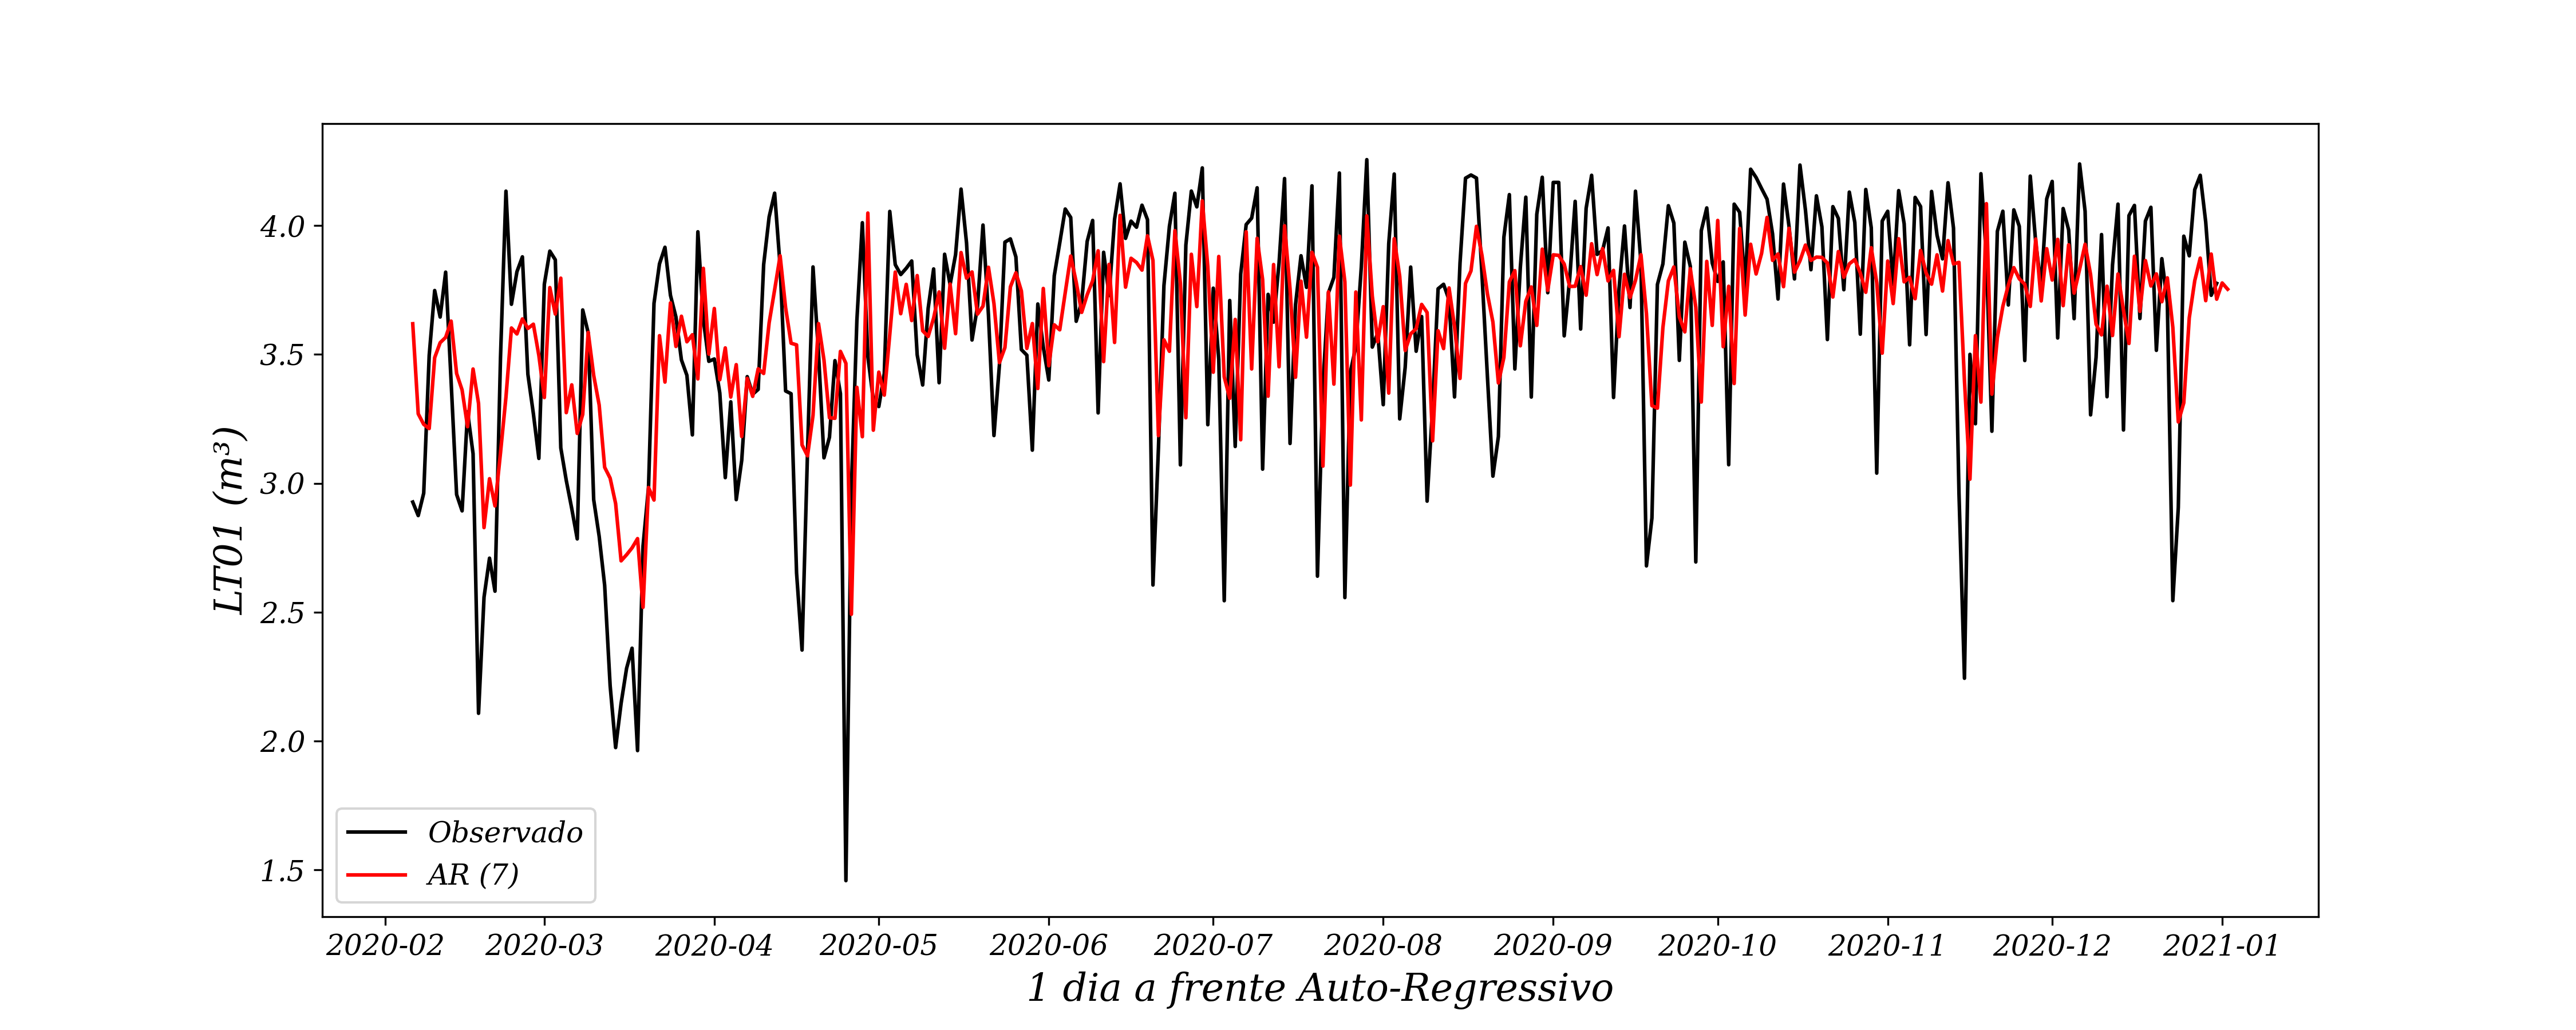
\includegraphics[width=1\linewidth]{Modelos/Figuras/1-AR}
	
	Fonte: Elaboração própria a partir de dados da SANEPAR (2018 a 2020)
\end{figure}

\begin{figure}[H]
	\centering
	\caption{ARX (7) com um passo a frente}
	\label{fig:1-arx}
	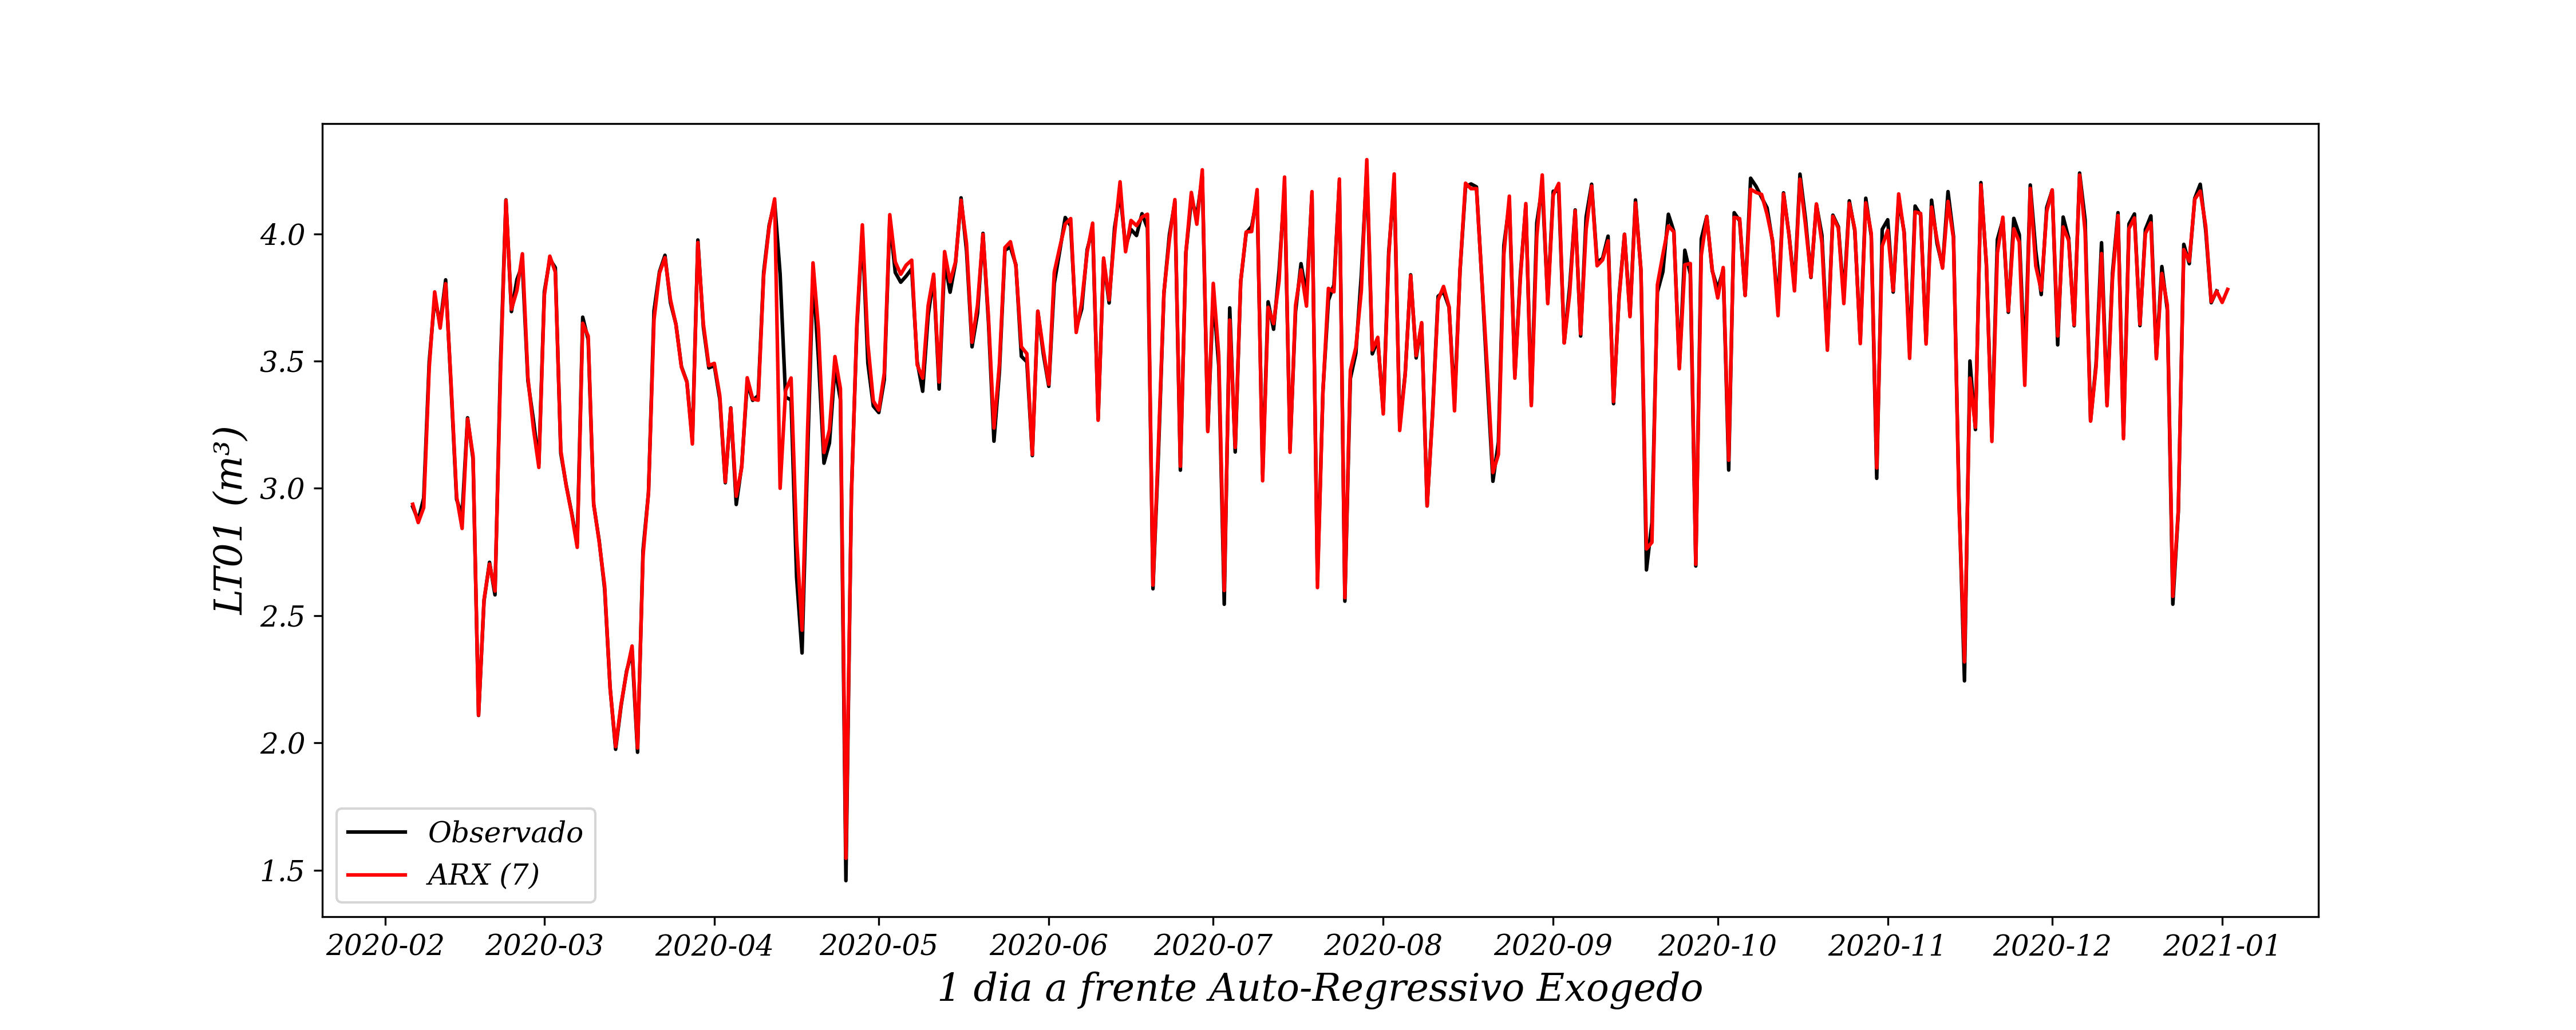
\includegraphics[width=1\linewidth]{Modelos/Figuras/1-ARX}
	
	Fonte: Elaboração própria a partir de dados da SANEPAR (2018 a 2020)
\end{figure}



Onde em \eqref{AR} o $\varepsilon_t$ é ruído branco. Isso é como uma regressão múltipla, mas com valores defasados de $y_t$ como preditores. é referido a isso como um $\operatorname{AR}(p)$ modelo, um modelo auto regressivo de ordem $p$

Da Figura \ref{fig:1-ar}, tem como objetivo mostrar uma previsão de um passo a frente (um dia) nos apêndices \ref{sec:ararxma18}, \ref{sec:ararxma24} pode ver uma comparação dos AR, MA e o ARX

O modelo ARX é um modelo similar ao AR só coloca as variáveis exógenas do conjunto de dados para melhorar a previsão futura.

O modelo AR pode ser visivelmente um modelo adequado para a previsão que está sendo feito, mas como é um modelo auto regressivo ainda assim com o passar do tempo e da previsão ele vai prever de uma forma linear e não convencional, para um analise mais rápido da série pode se considerar um modelo adequado. Logo mais adiante tem exemplos de casos gerais que pode ocorrer nesse método.

\textbf{AR(0): Ruído branco}

Se definir o parâmetro $p$ como zero (AR($0$)), sem termos autorregressivos. Esta série de tempo é apenas um ruído branco. Cada ponto de dados é amostrado a partir de uma distribuição com uma média de $0$ e uma variância de sigma-quadrado. Isso resulta em uma sequência de números aleatórios que não podem ser previstos. Isso é realmente útil, pois pode servir como uma hipótese nula, e proteger nossas análises de aceitar padrões falso-positivos.

\textbf{AR(1): Caminhadas aleatórias e Oscilações}



Com o parâmetro p definido para $1$, vai levar em conta o medidor de tempo anterior ajustado por um multiplicador e, em seguida, adicionando ruído branco. Se o multiplicador é $0$, então temos ruído branco, e se o multiplicador é 1, teremos uma caminhada aleatória. Se o multiplicador estiver entre $ 0 < \alpha < 1 $, então a série temporal exibirá reversão média. Isso significa que os valores tendem a pairar em torno de 0 e reverter para a média depois de regredir a partir dele.

\textbf{AR(p): Termos de ordem superior}

Aumentar ainda mais o parâmetro $p$ significa apenas ir mais para trás e adicionar mais medidores de tempo ajustados por seus próprios multiplicadores. Pode ir o mais longe que poder, mas à medida que aproxima é mais provável que usa parâmetros adicionais, como a média móvel (MA($q$)).

\subsubsection{Média Móvel — MA(q)}\label{subsubsec:ma}
Este componente não é uma média de rolamento, mas sim os atrasos no ruído branco. \citeonline{signal}


MA(q) é o modelo de média móvel e q é o número de termos de erro de previsão defasados na previsão. Em um modelo MA(1), na previsão é um termo constante mais o termo de ruído branco anterior vezes um multiplicador, adicionado com o termo de ruído branco atual. Esta é apenas simples probabilidade mais estatísticas, pois estamos ajustando nossa previsão com base em termos anteriores de ruído branco.

\begin{eqnarray}
	y_t=c+\varepsilon_t+\theta_1 \varepsilon_{t-1}+\theta_2 \varepsilon_{t-2}+\cdots+\theta_q \varepsilon_{t-q}\label{eq:ma}
\end{eqnarray}

De \eqref{eq:ma} onde $\varepsilon_t$ é ruído branco. Refere nos a isto como um modelo de $MA(q)$, um modelo de ordem média móvel $q$. Claro que não observamos os valores de $\varepsilon_t$, por isso não é realmente uma regressão no sentido habitual.

\begin{figure}[H]
	\centering
	\caption{Modelo MA(7) com um passo a frente}
	\label{fig:1-ma}
	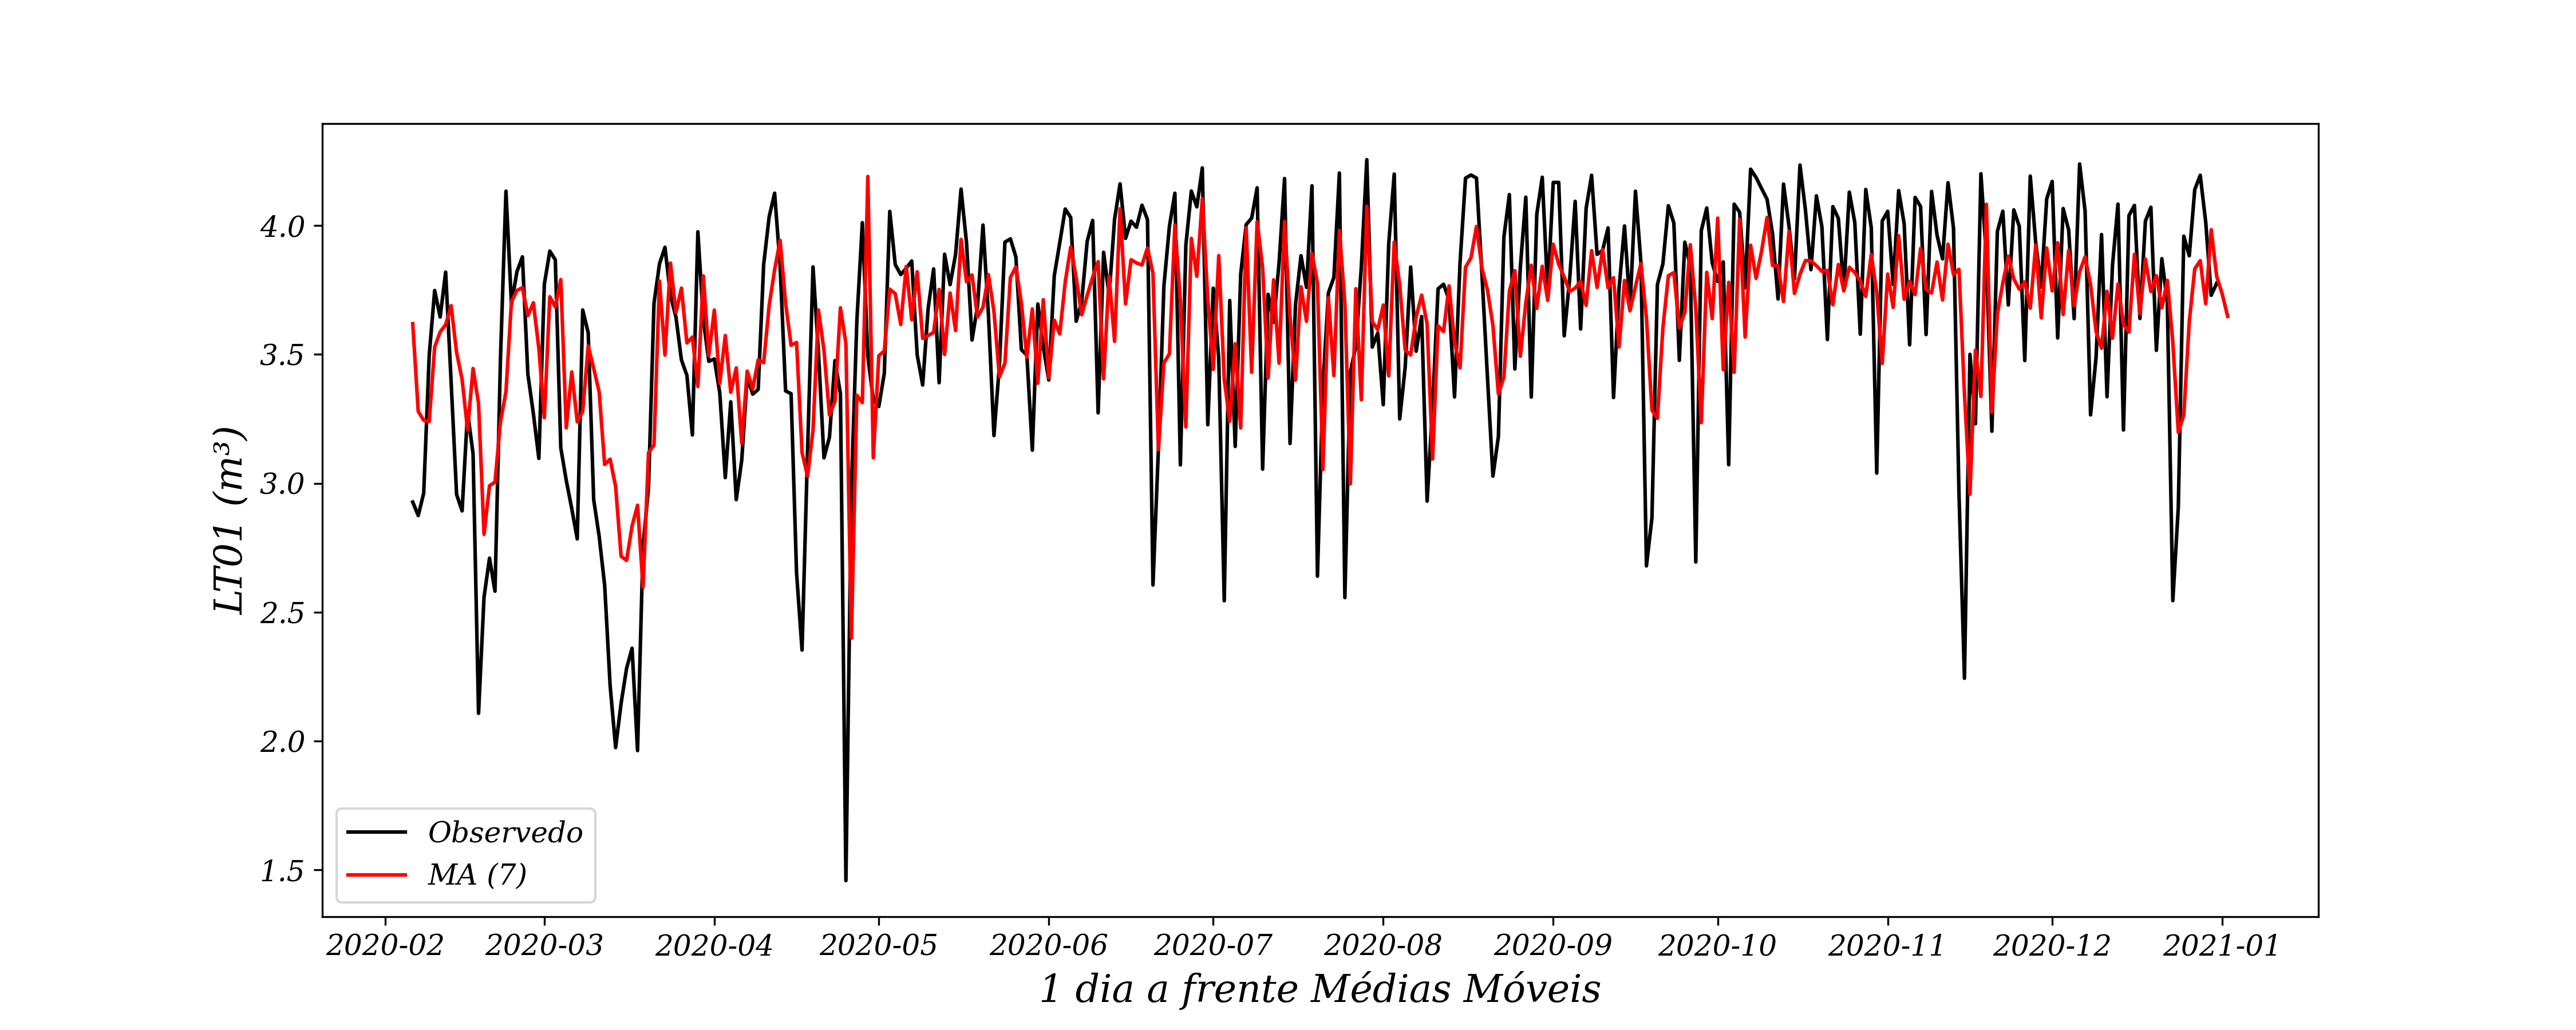
\includegraphics[width=1\linewidth]{Modelos/Figuras/1-MA}
	
	Fonte: Elaboração própria a partir de dados da SANEPAR (2018 a 2020)
\end{figure}

O modelo MA com o mesmo valor do AR para comparação e torna o modelo mais fácil de ser previsto. Como observado na Figura \ref{fig:1-ma} a previsão graficamente é parecido com o modelo da Figura \ref{fig:1-ar}, só não se compara com a Figura \ref{fig:1-arx}, perceba que esse modelo aparente prever perfeitamente o tempo que foi listado.  

\subsubsection{Modelos ARMA e ARIMA}\label{subsubsec:arma}
As arquiteturas ARMA e ARIMA são apenas os componentes AR (Autoregressive) e MA (Moving Average) juntos.

\textbf{ARMA}

O modelo ARMA é uma constante mais a soma de lags AR e seus multiplicadores, além da soma dos lags ma e seus multiplicadores mais ruído branco. Esta equação é a base de todos os modelos que vêm a seguir e é uma estrutura para muitos modelos de previsão em diferentes domínios.

\begin{figure}[H]
	\centering
	\caption{ARMA (7,7) com um passo a frente}
	\label{fig:1-arma}
	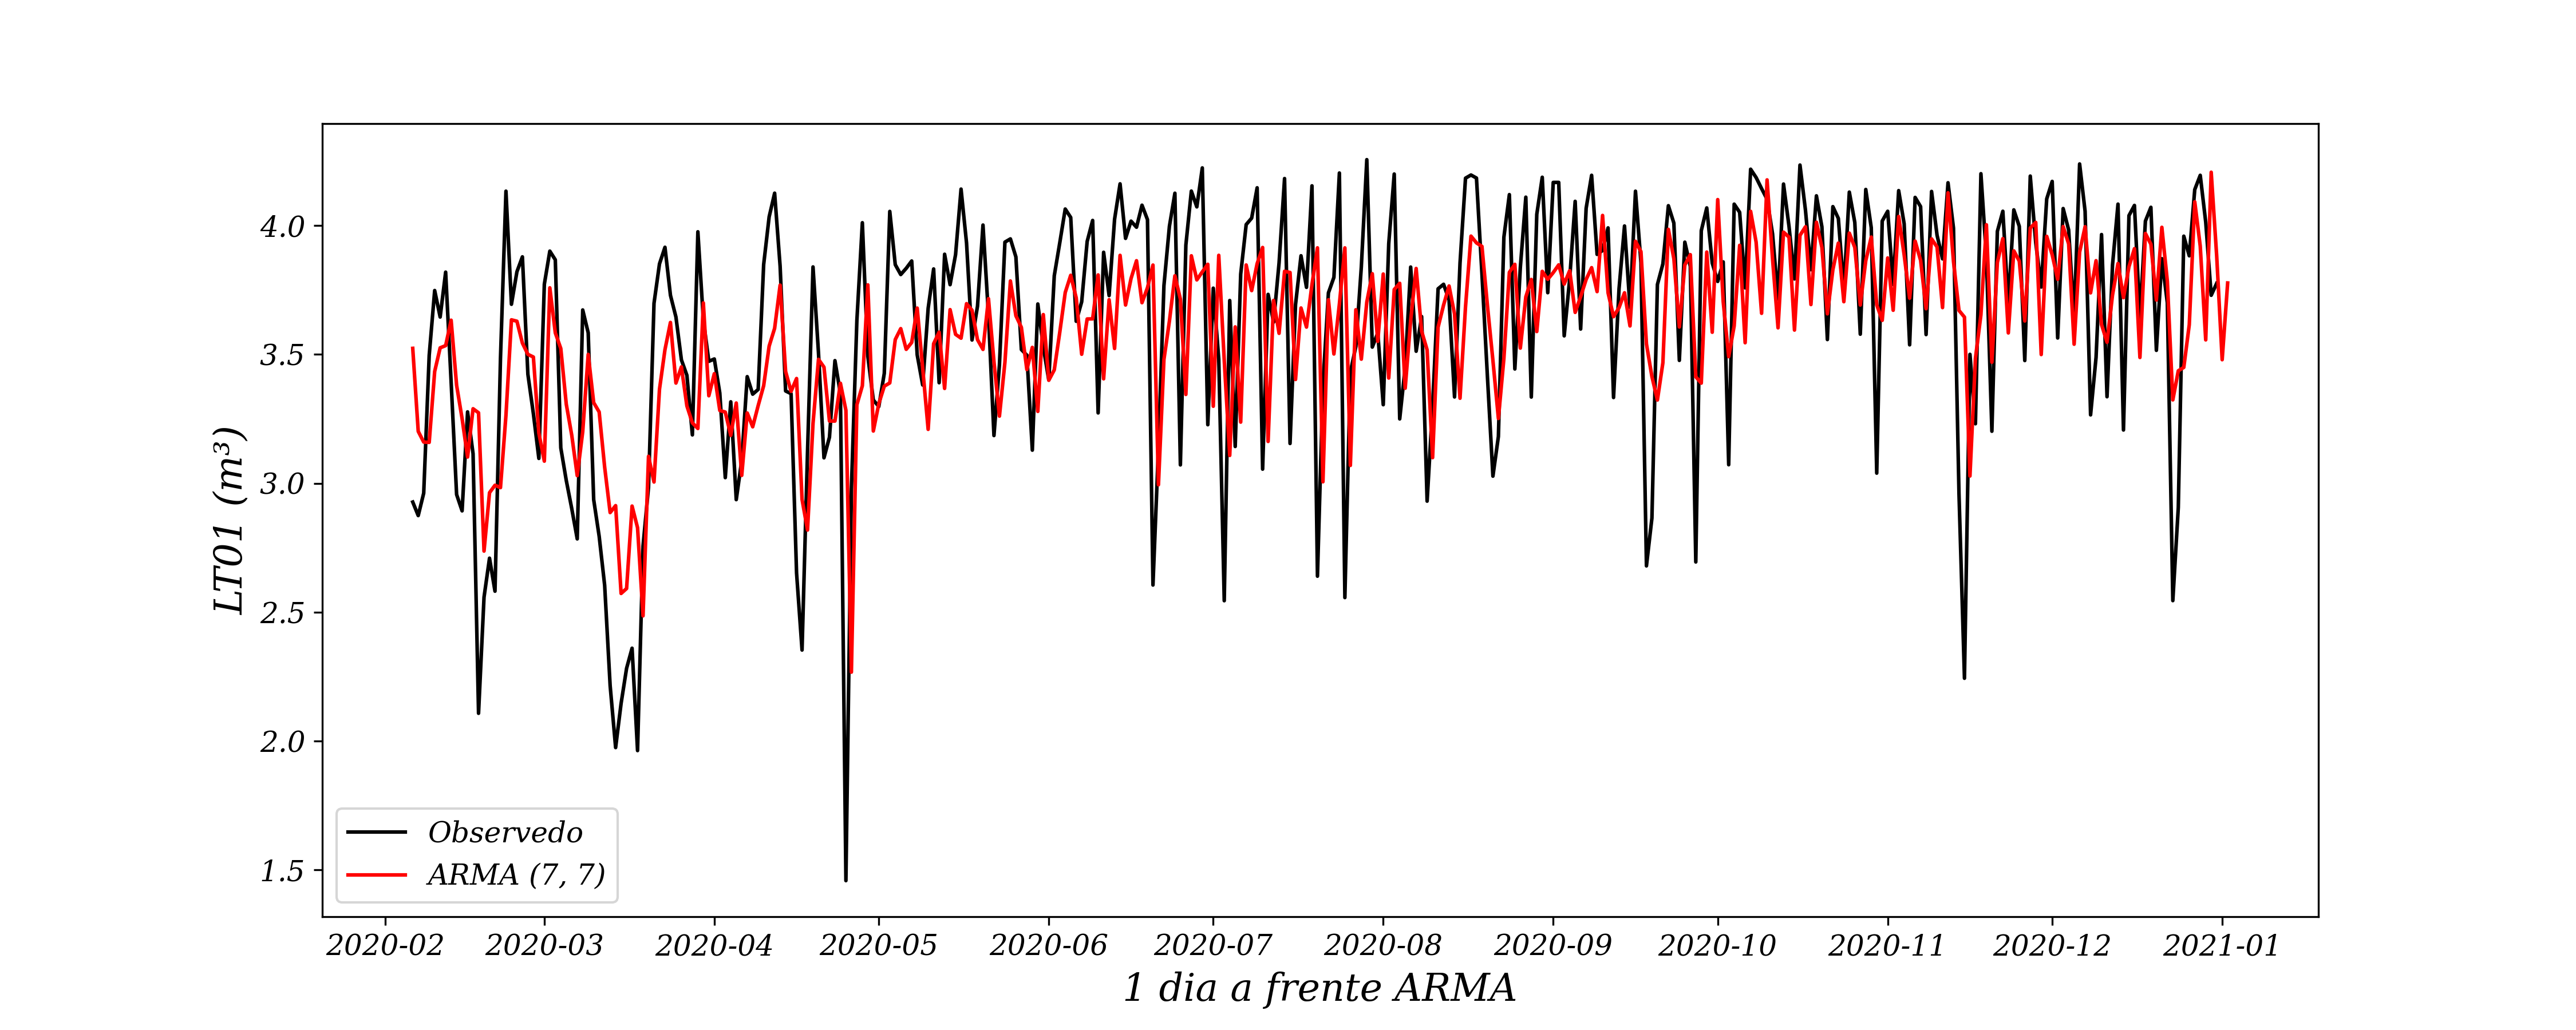
\includegraphics[width=1\linewidth]{Modelos/Figuras/1-ARMA}
	
	Fonte: Elaboração própria a partir de dados da SANEPAR (2018 a 2020)
\end{figure}

Da Figura \ref{fig:1-arma} é a junção dos modelos AR e MA esse modelos juntos pode ocorrer a redução do erro em escala mais significativa, nos apêndice \ref{sec:comtb24} e \ref{sec:comtb18} pode ser notado a comparação de alguns passos a mais do que mostrado aqui.

\textbf{ARIMA}

\begin{eqnarray}
	Y_t = \beta_2 + \omega_1\varepsilon_{t-1} + \omega_2 \varepsilon_{t-2} +\ldots+ \omega_q \varepsilon_{t-q} + \varepsilon_t \label{arima}
\end{eqnarray}


Onde em \eqref{arima} o $Y_t$ é a série diferenciada (pode ter sido diferente mais de uma vez). Os ``preditores" no lado direito incluem ambos os valores defasados de $Y_t e$ erros defasados. Chamamos isso de ARIMA( $p, d, q$ ).

O modelo ARIMA é um modelo ARMA ainda com uma etapa de pré-processamento incluída no modelo que representamos usando I(d). I(d) é a ordem de diferença, que é o número de transformações necessárias para tornar os dados estacionários. Assim, um modelo ARIMA é simplesmente um modelo ARMA na série de tempo diferente.

\begin{figure}[H]
	\centering
	\caption{ARIMA (7,1,7) com um passo a frente}
	\label{fig:1-arima}
	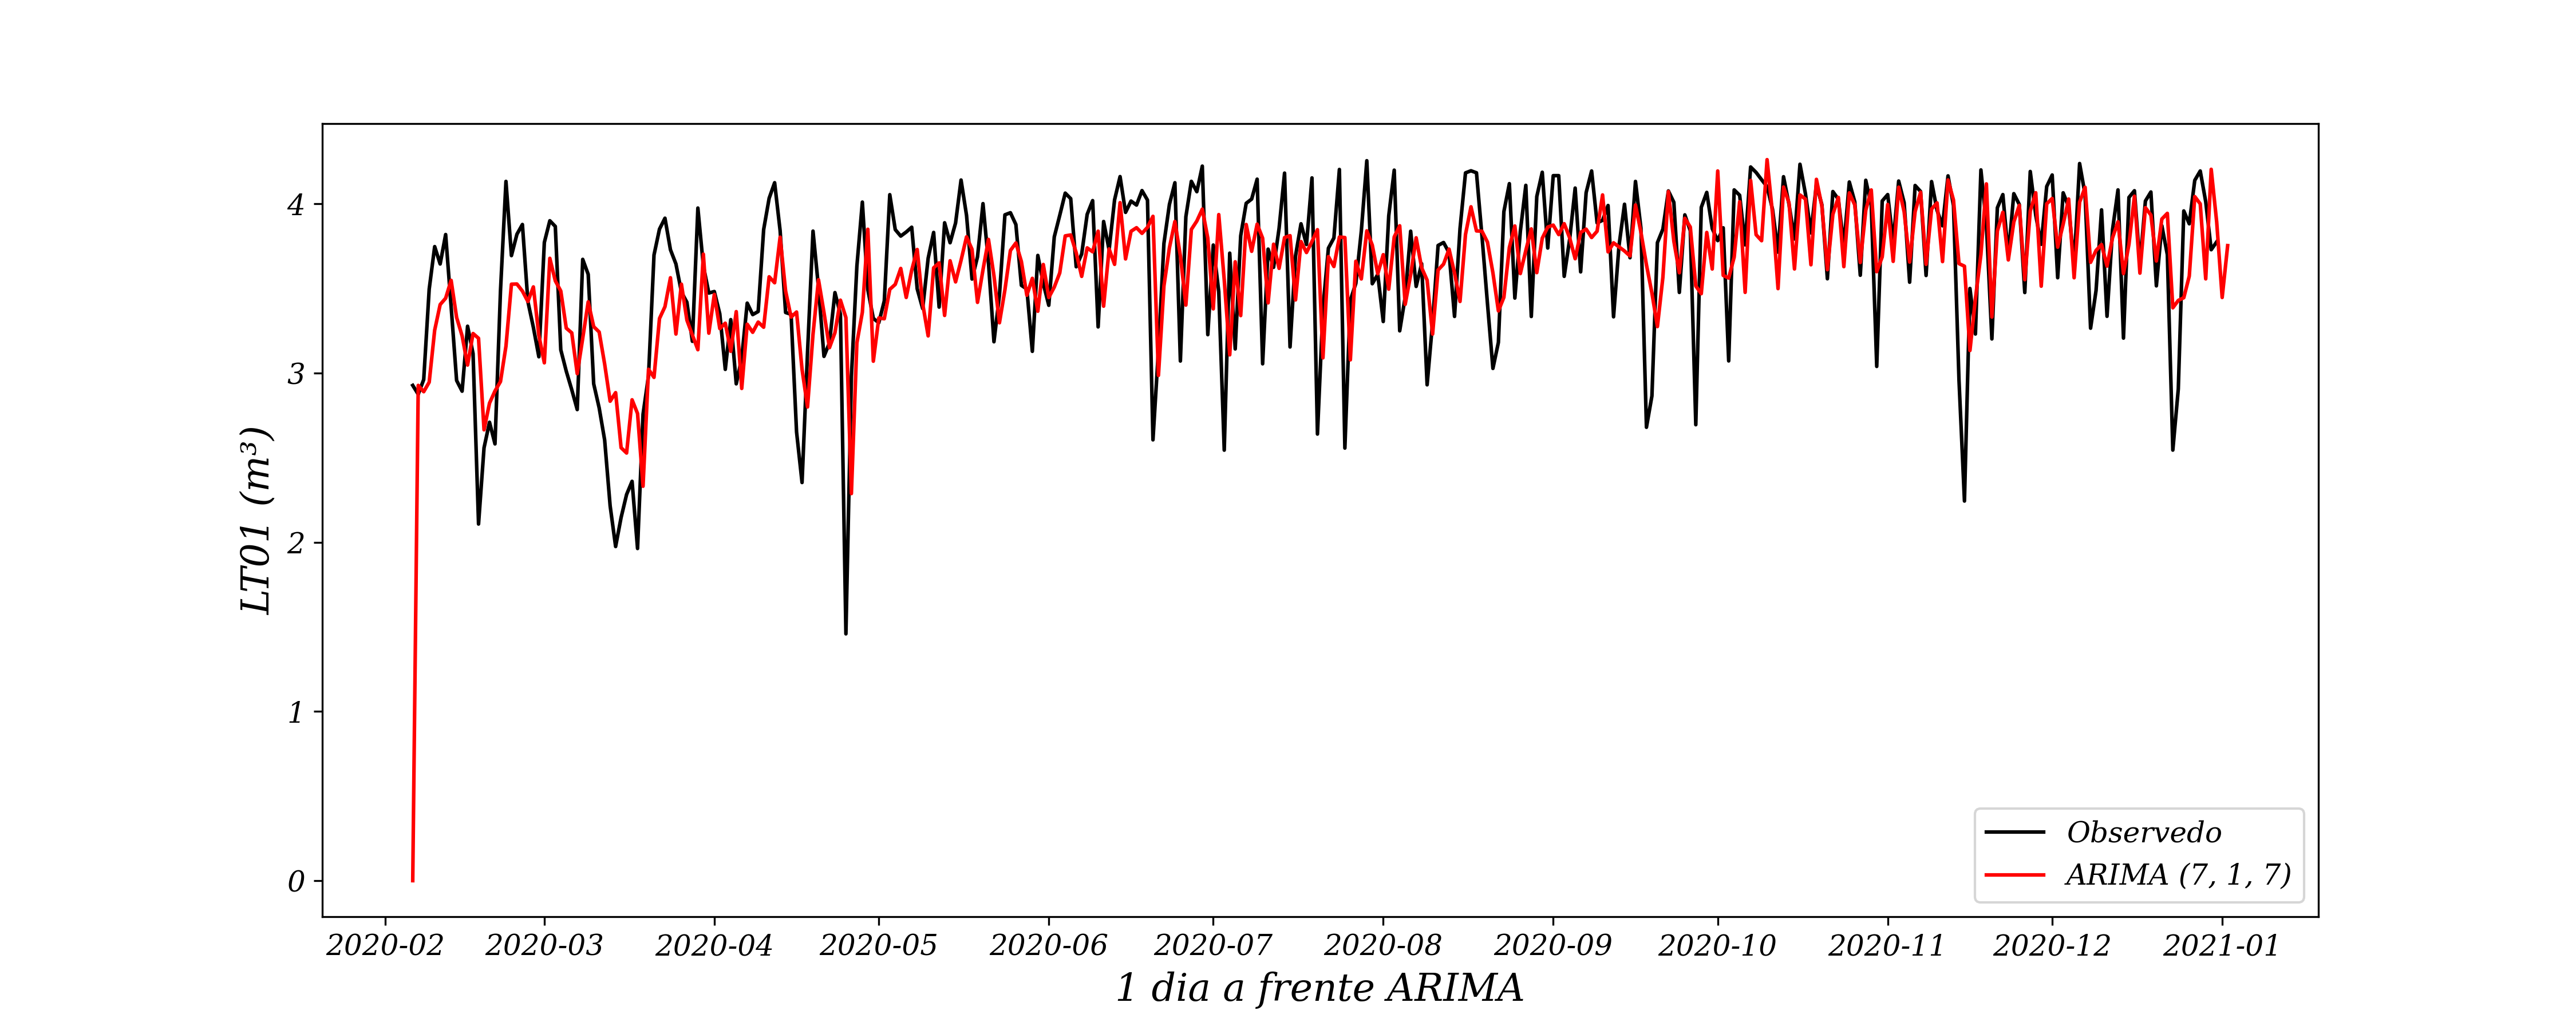
\includegraphics[width=1\linewidth]{Modelos/Figuras/1-ARIMA}
	
	Fonte: Elaboração própria a partir de dados da SANEPAR (2018 a 2020)
\end{figure}

Olhando a Figura \ref{fig:1-arima} podemos perceber que não tem muita diferença visual com os outros métodos mostrados até agora, visualmente o método ARX ainda esta melhor que os outros.  


\subsubsection{MODELOS SARIMA, ARIMAX, SARIMAX}

Os modelos ARIMA são ótimos, mas incluir variáveis sazonais e exógenas no modelo pode ser muito poderoso. Como o modelo ARIMA assume que a série temporal é estacionária, precisamos usar um modelo diferente.
\textbf{SARIMA}

\begin{eqnarray}
	Y_t&=&c+\sum_{n=1}^p \alpha_n y_{t-n}+\sum_{n=1}^q \theta_n \epsilon_{t-n}+\sum_{n=1}^P \phi_n y_{t-s n}+\sum_{n=1}^Q \eta_n \epsilon_{t-s n}+\epsilon_t \label{sarima}
\end{eqnarray}

O modelo é muito semelhante ao modelo ARIMA, com um conjunto adicional de componentes autorregressivos e de média móvel. O atraso extra é compensado pela frequência sazonal (por exemplo, 12 - mensal, 24 - por hora). 

\begin{figure}[H]
	\centering
	\caption{SARIMA $(7,1,7) (2,1,1)_{12}$}
	\label{fig:1-sarima}
	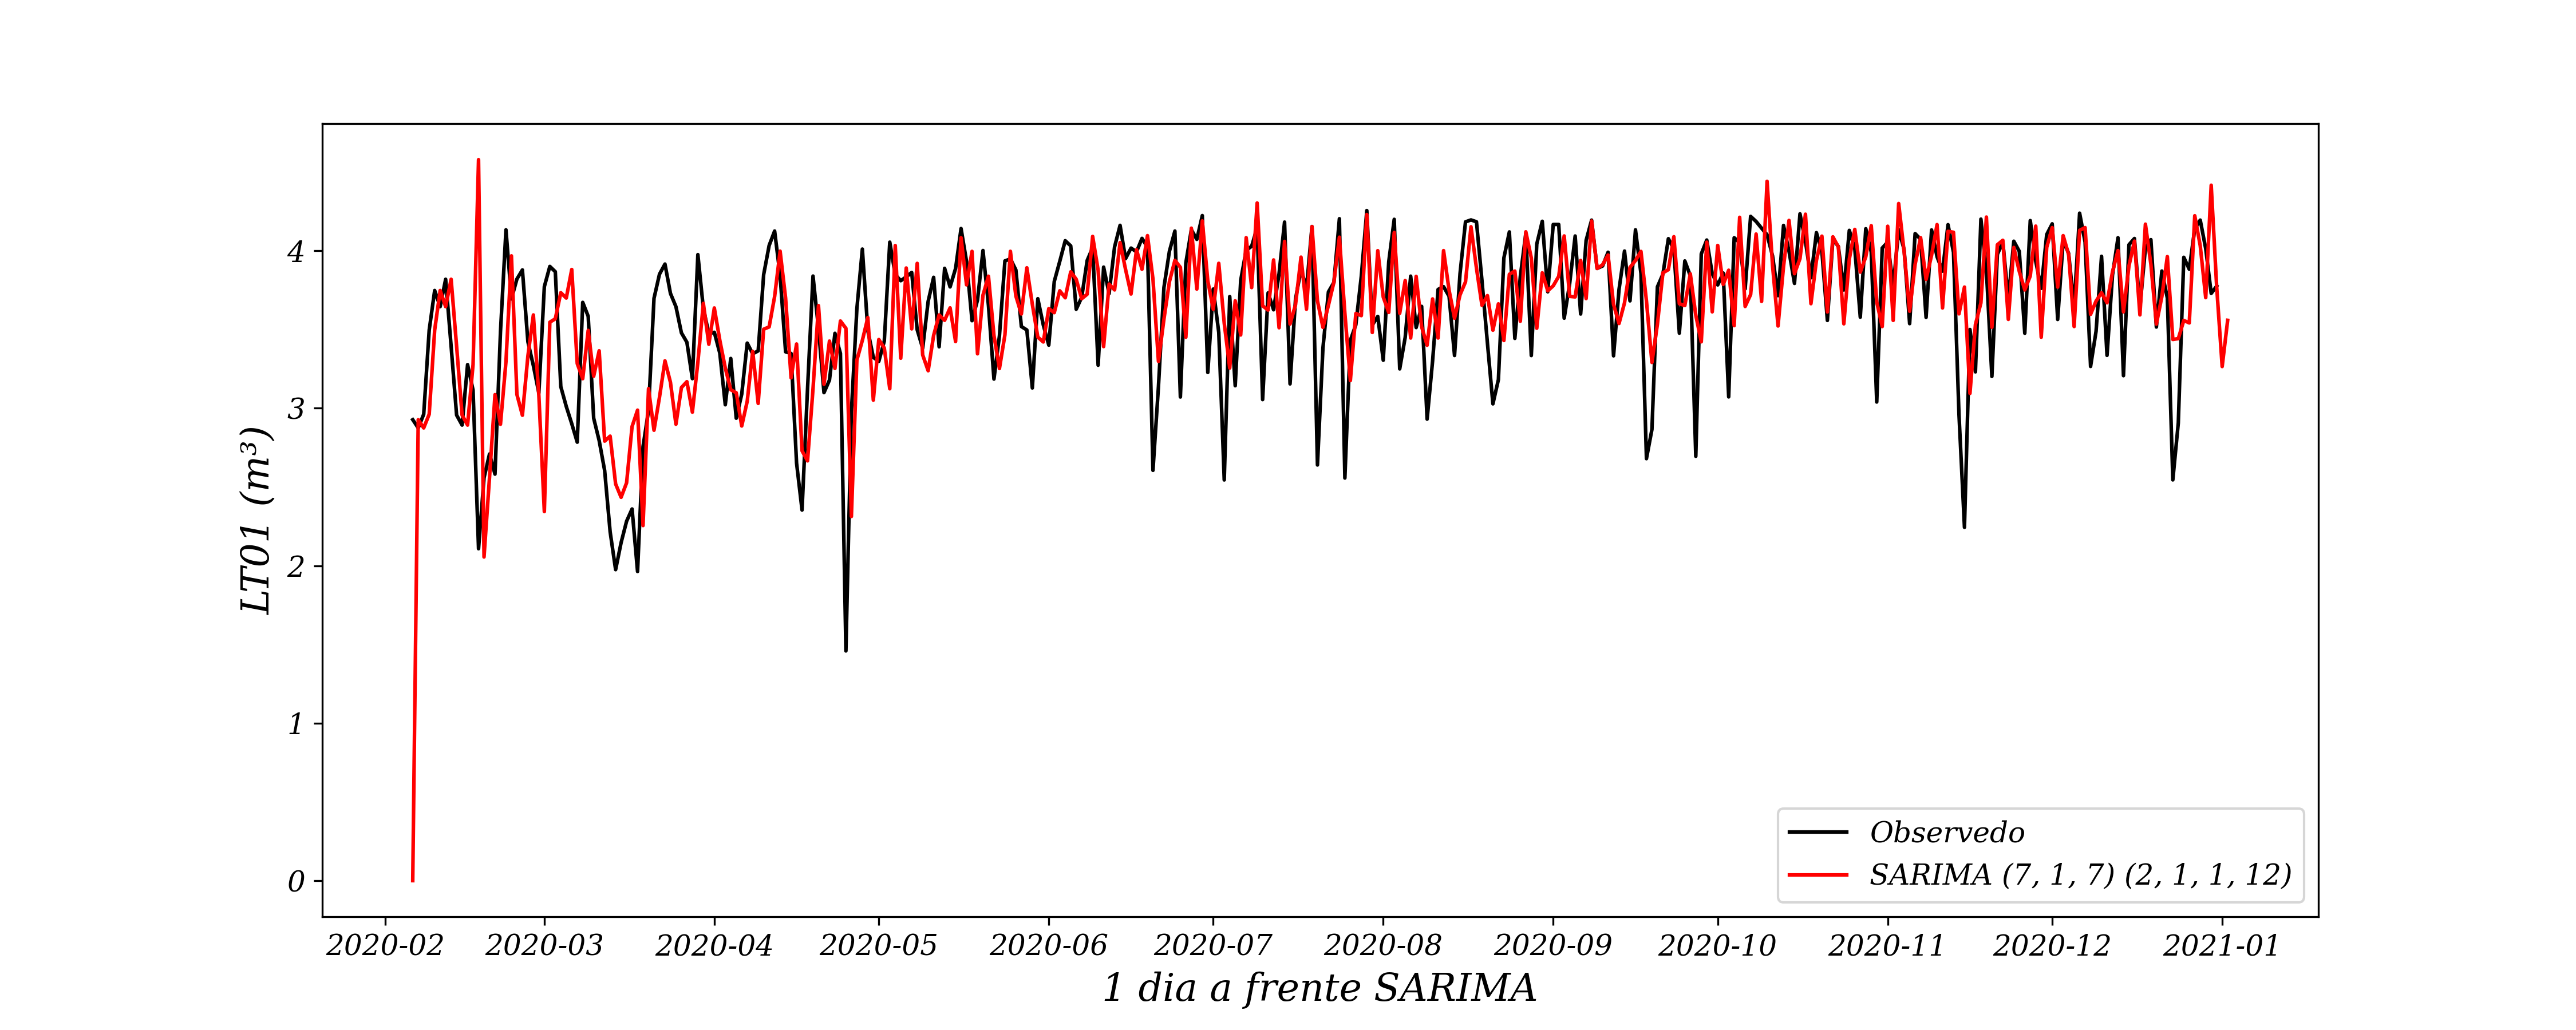
\includegraphics[width=1\linewidth]{Modelos/Figuras/1-SARIMA}
	
	Fonte: Elaboração própria a partir de dados da SANEPAR (2018 a 2020)
\end{figure}

Na Figura \ref{fig:1-sarima} pode ser observado como a previsão em vermelho esta mais próxima do observado em preto, só acionando o termo de sazonalidade na previsão. 

Os modelos SARIMA permitem diferenciar dados por frequências sazonais e não sazonais. Uma estrutura de pesquisa automatizada de parâmetros, como pmdarina, pode ajudar a entender quais são os melhores parâmetros.

\textbf{ARIMAX e SARIMAX}

\begin{eqnarray}
	d_t=c+\sum_{n=1}^p \alpha_n d_{t-n}+\sum_{n=1}^q \theta_n \epsilon_{t-n}+\sum_{n=1}^r \beta_n x_{n_t}+\sum_{n=1}^P \phi_n d_{t-s n}+\sum_{n=1}^Q \eta_n \epsilon_{t-s n}+\epsilon_t \label{eq:sarmax}
\end{eqnarray}

Em \eqref{eq:sarmax} está o modelo SARIMAX. Este modelo tem em conta variáveis exógenas, ou por outras palavras, utiliza dados externos na nossa previsão. É interessante pensar que todos os factores exógenos ainda são tecnicamente indiretamente modelados na previsão histórica do modelo. Dito isto, se incluirmos dados externos, o modelo responderá muito mais rapidamente ao seu efeito do que se confia na influência de termos desfasados.

\begin{figure}[H]
	\centering
	\caption{ARIMAX $(7,1,7)$ com um passo a frente}
	\label{fig:1-arimax}
	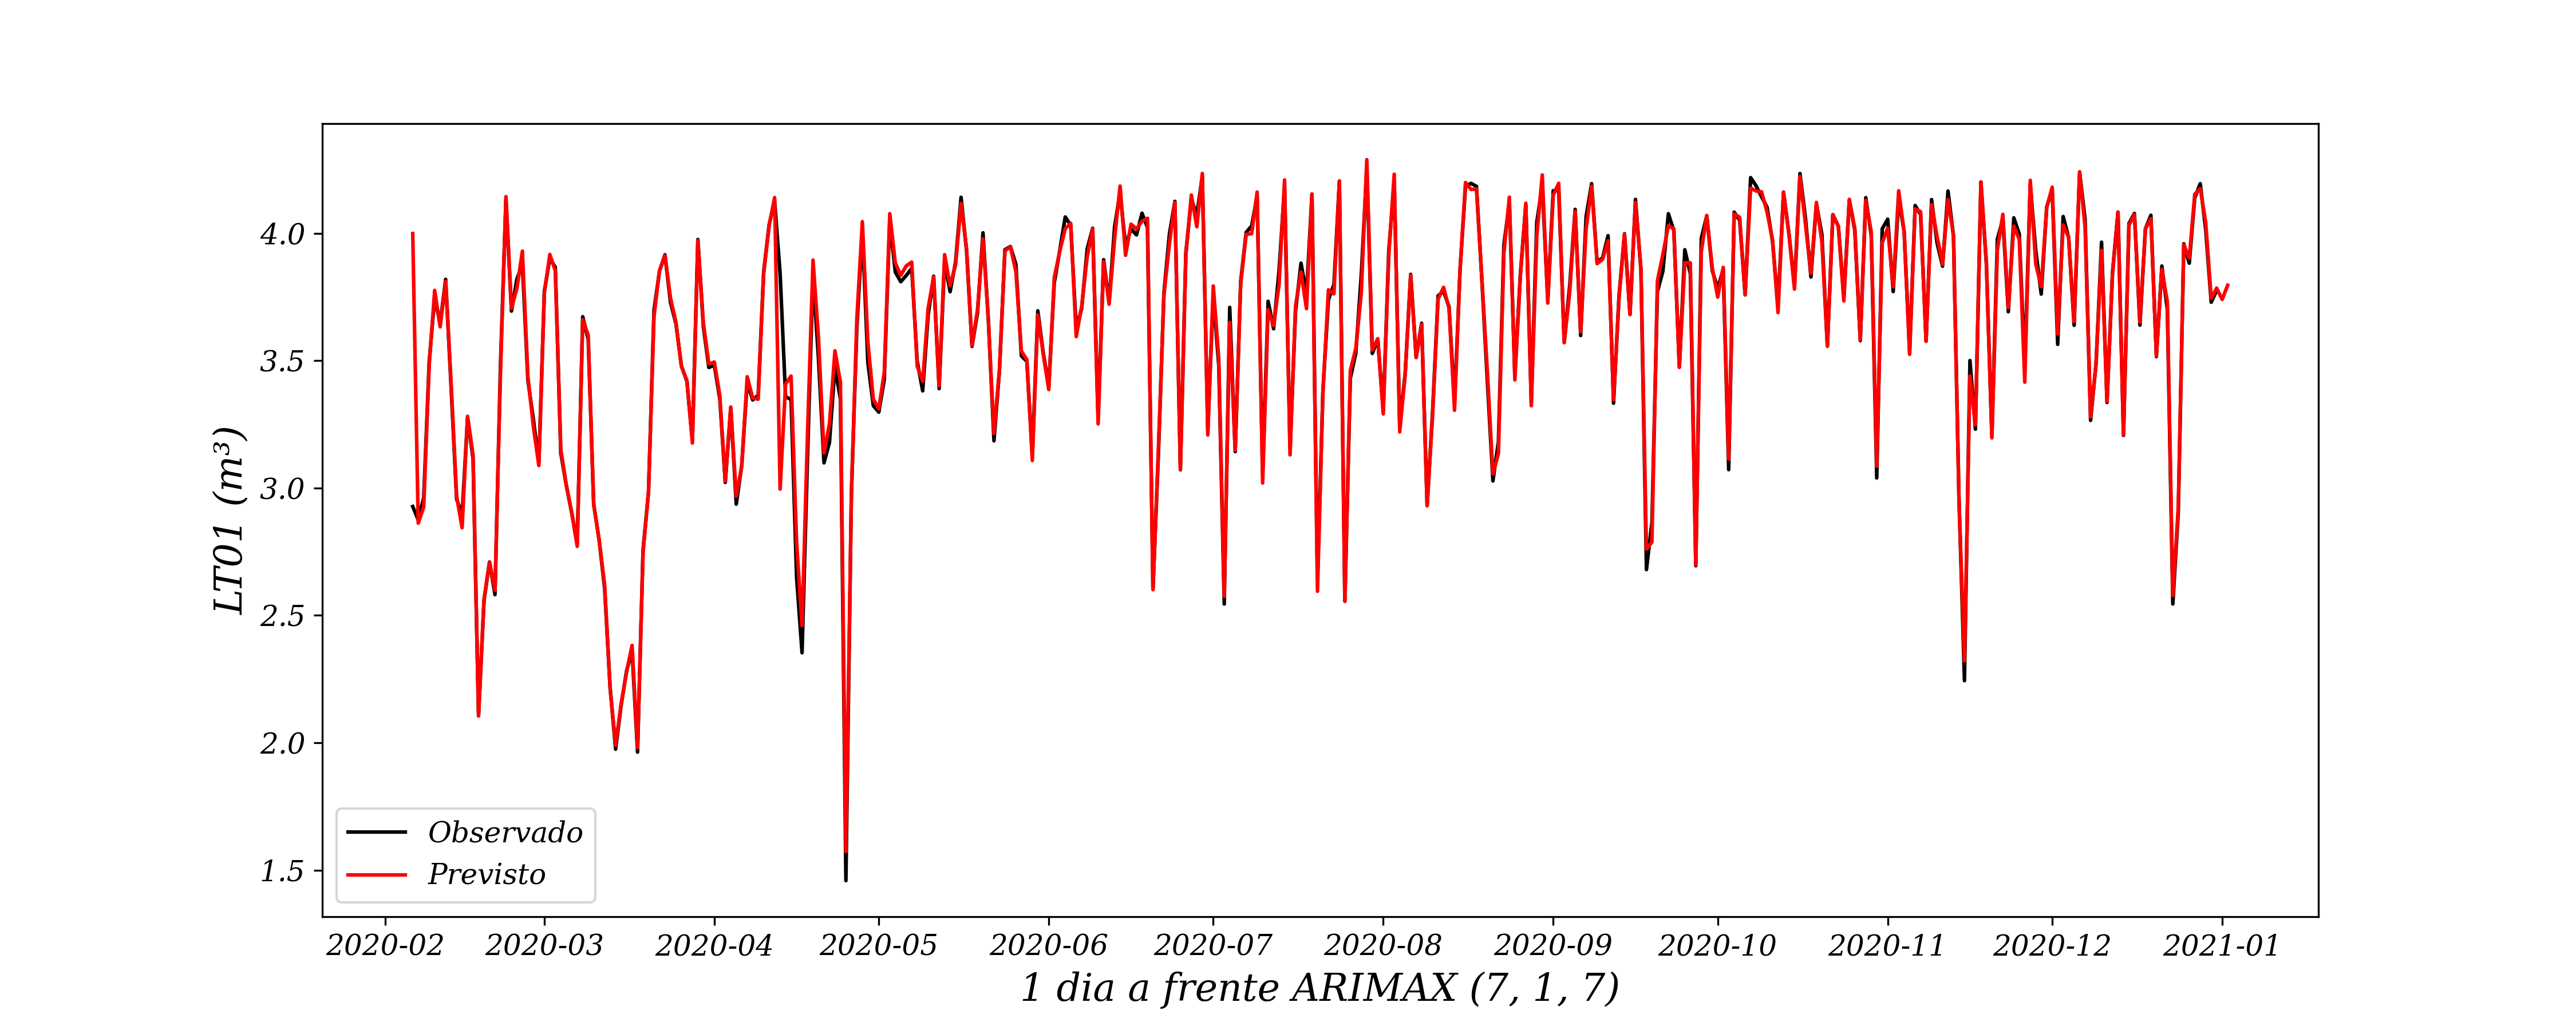
\includegraphics[width=1\linewidth]{Modelos/Figuras/1-ARIMAX}
	
	Fonte: Elaboração própria a partir de dados da SANEPAR (2018 a 2020)
\end{figure}

\begin{figure}[H]
	\centering
	\caption{SARIMAX $(7,1,7) (2,1,1)_{12}$ com um passo a frente}
	\label{fig:1-sarimax}
	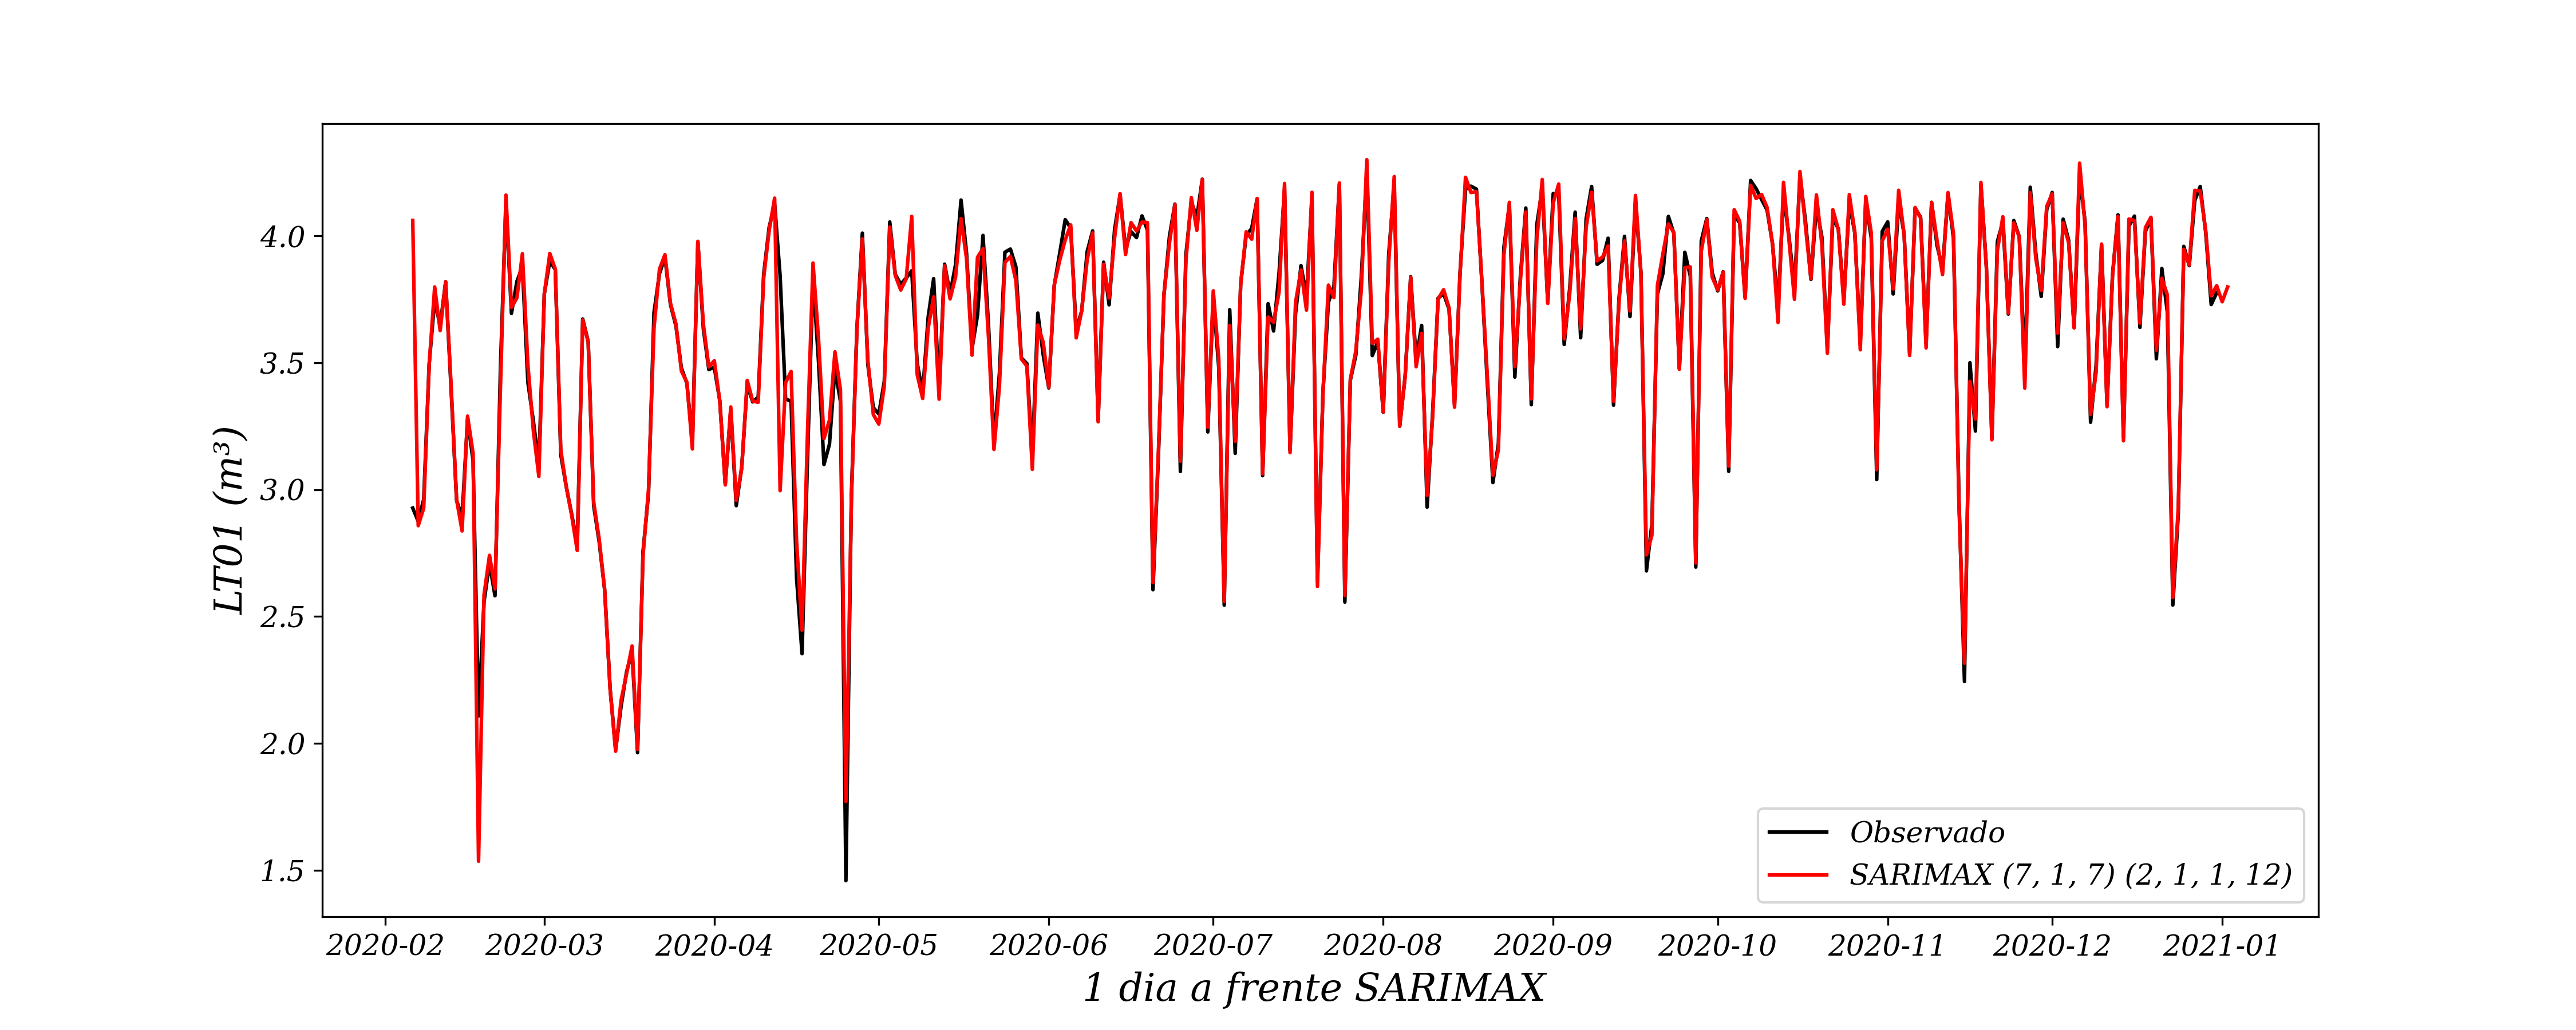
\includegraphics[width=1\linewidth]{Modelos/Figuras/1-SARIMAX}
	
	Fonte: Elaboração própria a partir de dados da SANEPAR (2018 a 2020)
\end{figure}


Entre os modelos com variáveis exógenas os modelos da Figura \ref{fig:1-arimax} e \ref{fig:1-sarimax}, é possível perceber que a previsão está mais completa do que nos modelos sem a variável exógena.

\subsection{Modelos Regressivo}\label{subsec:reg}

\subsubsection{Regressão Linear (LR)}

Segundo \citeonline{korstanje2021} nos modelos de aprendizado de máquina supervisionados, você tenta identificar relações entre diferentes variáveis:

\begin{itemize}
	\item Variável de destino: a variável que você tenta prever
	\item Variáveis explicativas: Variáveis que ajudam você a prever o alvo variável
\end{itemize}

Para a previsão, é importante entender quais tipos de variáveis explicativas você pode ou não usar. Como exemplo, aqui vai ser usado as variáveis \textbf{Pressão de Succção (PT01SU)} como variável $x$ e \textbf{Nível do Reservatório (Câmara 1) LT01} como variável $y$ pois na correlação de Pearson mostrado na Figura \ref{fig:person}, o coeficiente mostra a relação que tem entre o eixo $x$ e $y$ com a seguinte fórmula.



\begin{eqnarray}
	r=\frac{\sum\left(x_i-\bar{x}\right)\left(y_i-\bar{y}\right)}{\sqrt{\left(\sum\left(x_i-\bar{x}\right)^2\right)\left(\sum\left(y_i-\bar{y}\right)^2\right)}}\label{eq:pearson}
\end{eqnarray}
De \eqref{eq:pearson} sejam $x_i \in y_i$ os valores das variáveis $X$ e $Y$.  $\bar{x}$ e $\bar{y}$ são respectivamente as médias dos valores $x_i \in y_i$.

A fórmula do coeficiente de correlação de Pearson é então,

\begin{figure}[H]
	\centering
	\caption{Corelação de Pearson }
	\label{fig:person}
	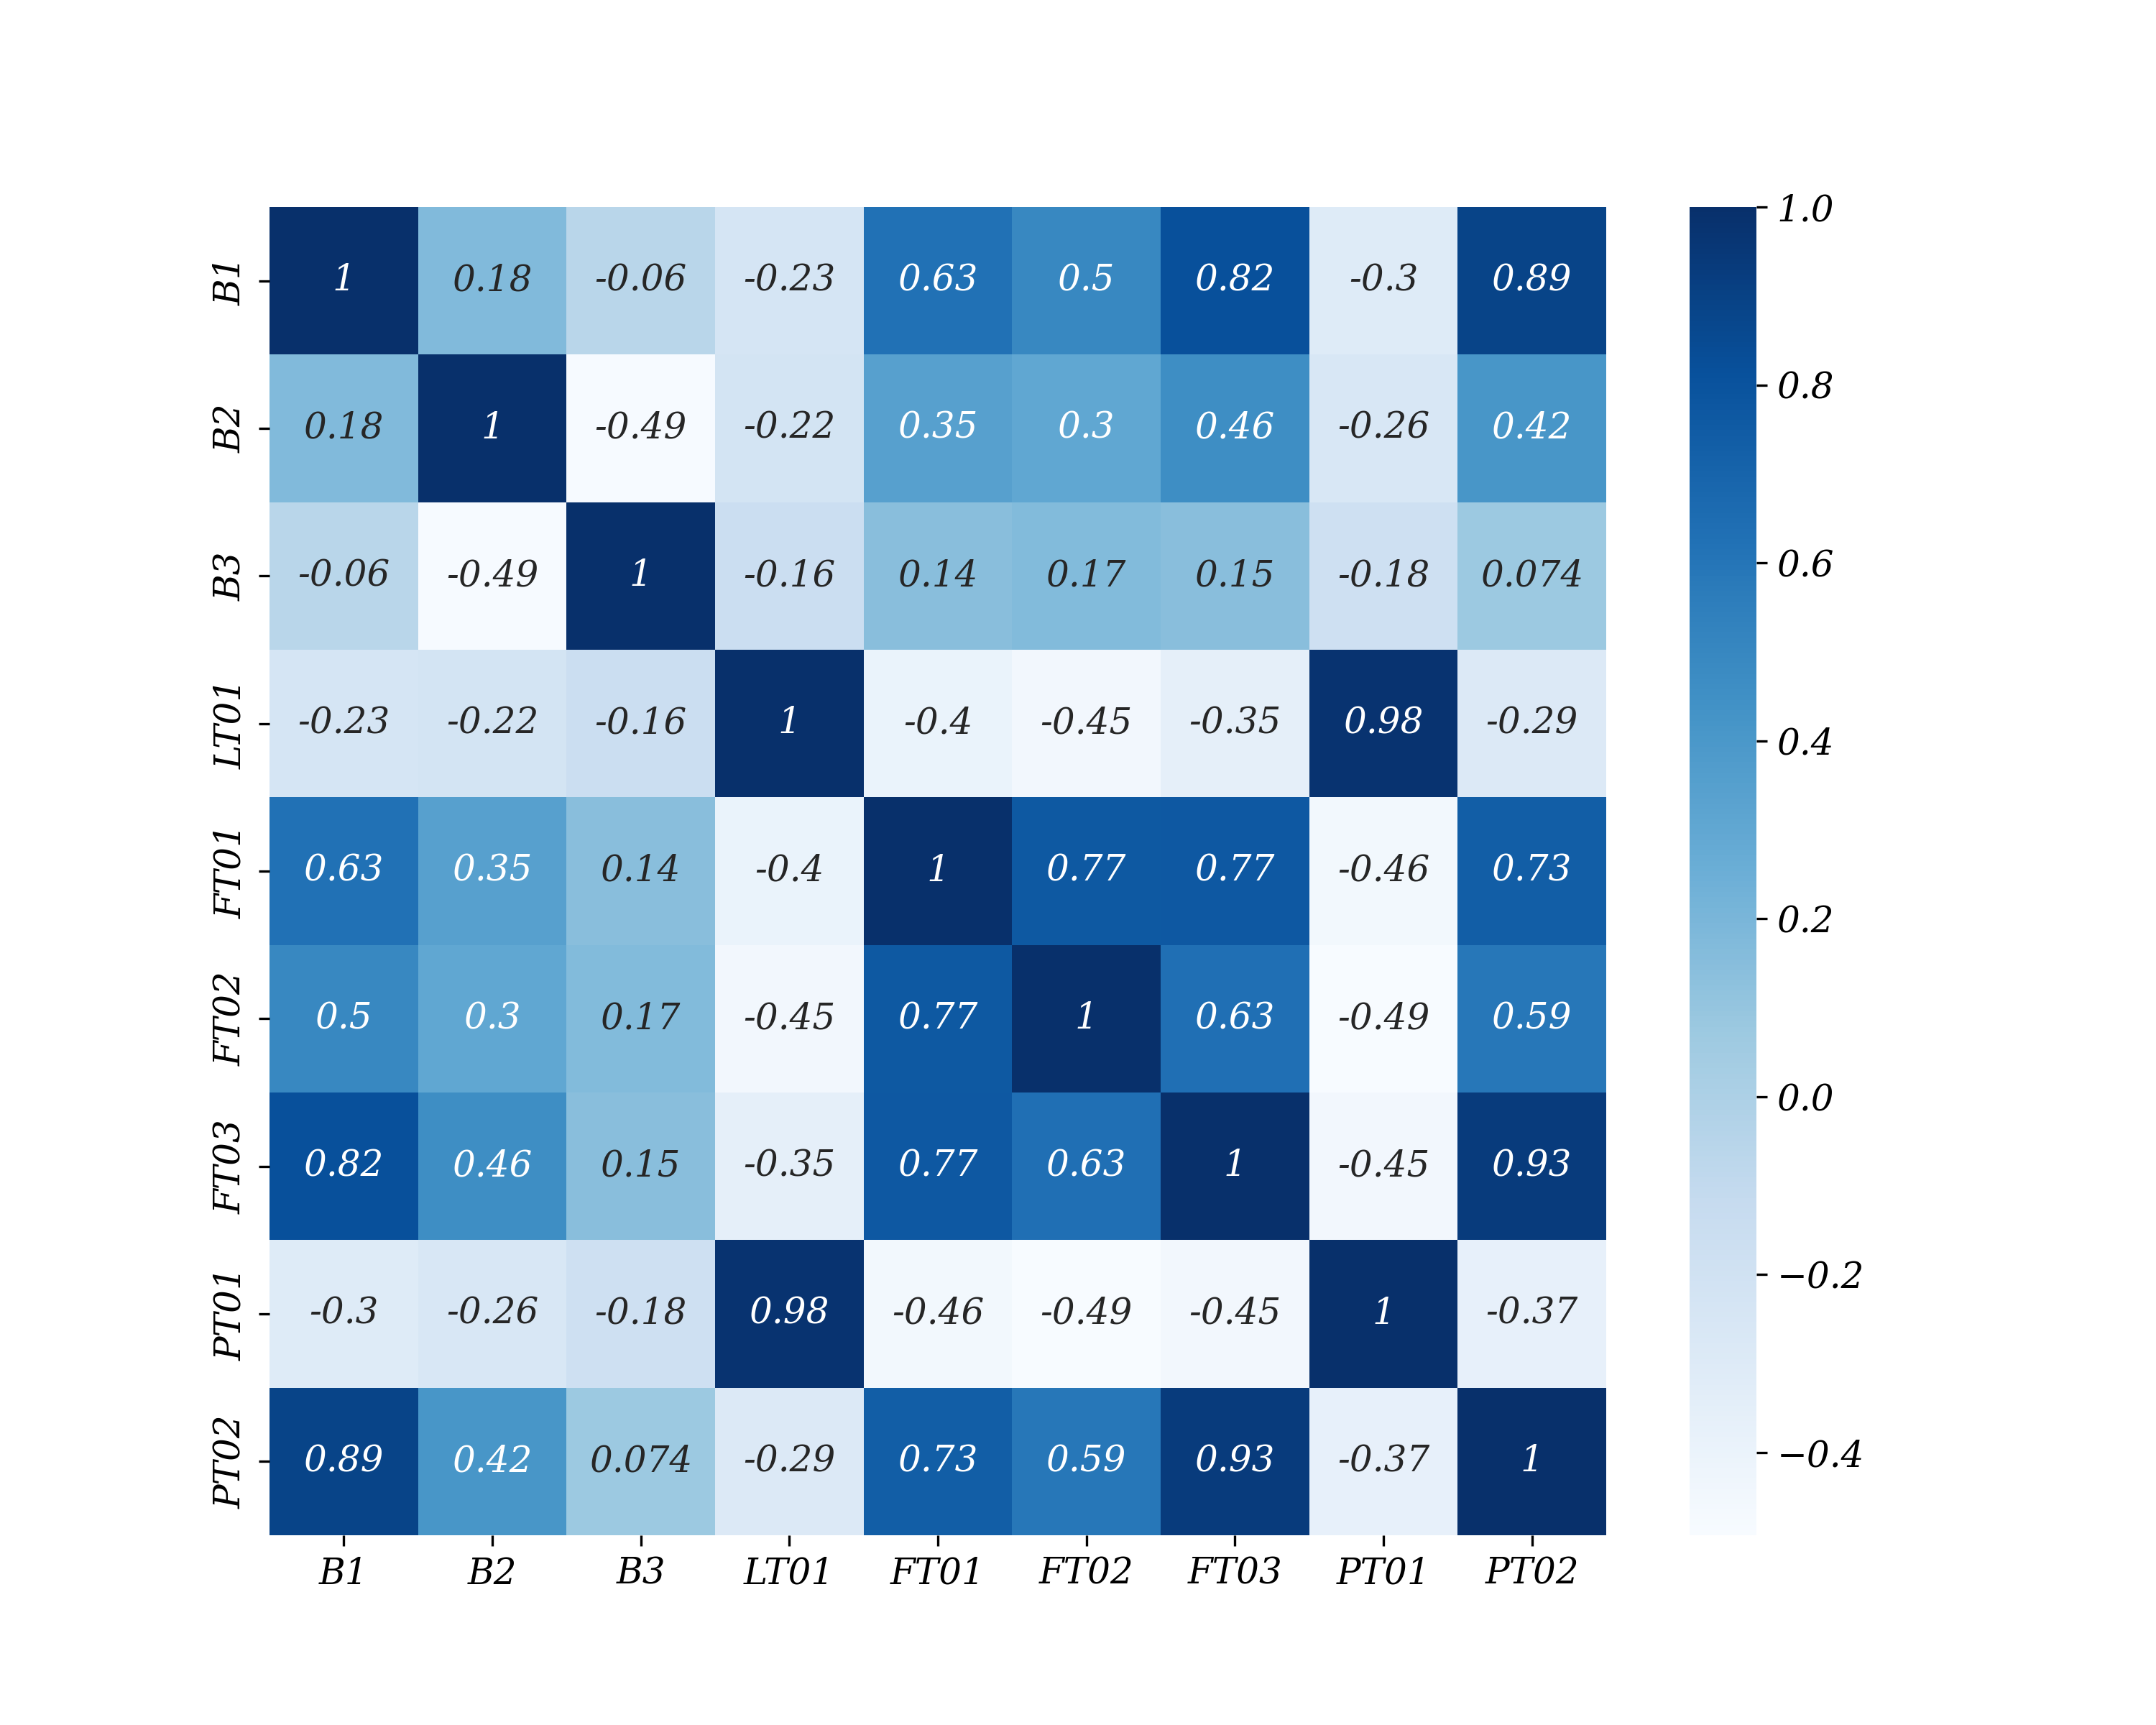
\includegraphics[width=1\linewidth]{Apendices/Figuras/modelagem-24h/person}
	
	Fonte: Elaboração própria a partir de dados da SANEPAR (2018 a 2020)
\end{figure}

Como mostra a Figura \ref{fig:person} essa imagem é meramente ilutação da correlação que tem relação no conjunto de dados que esta sendo trabalhado aqui. E com isso também pode ser respondido a \ref{q1} da pesquisa. porque a correlação entre essas variáveis é forte.

\textbf{Definição do modelo}

A regressão linear é definida da seguinte forma:
\begin{eqnarray}
y&=&\beta_0+\beta_1 x_1+\cdots+\beta_p x_p+\varepsilon\label{eq:lr}
\end{eqnarray}
Da \eqref{eq:lr} têm a seguinte variáveis:

\begin{itemize}
	\item  Há $p$ variáveis explicativas, chamadas $x$.
\item Existe uma variável alvo chamada $y$.
\item  O valor para $y$ é calculado como uma constante $\left(\beta_0\right)$ mais os valores do $x$ variáveis multiplicadas pelos seus coeficientes $\beta_1$ para $\beta_p$.
\end{itemize}

\begin{figure}[H]
	\centering
	\caption{Regressão linear LT01 vs PT01 correlação 98\%}
	\label{fig:lr-lt01-m3}
	\includegraphics[width=1\linewidth]{"Modelos/Figuras/LR LT01 (m³)"}
	
	Fonte: Elaboração própria a partir de dados da SANEPAR (2018 a 2020)
\end{figure}



A Figura \ref{fig:lr-lt01-m3} mostra como interpretar $\beta_0$ e $\beta_1$ visualmente. Mostra que para um aumento de $1$ na variável $x$, o aumento na variável $x$ representa $\beta_1$. O valor para $0$ é o valor para $x$ quando $y$ é $0$.

Para poder utilizar a regressão linear, é necessário estimar os coeficientes (betas) sobre um conjunto de dados de formação. Os coeficientes podem então ser estimados utilizando a seguinte fórmula, em notação matricial:

\begin{eqnarray}
	\hat{\beta}&=&\left(X^T X\right)^{-1} X^T y\label{eq:ols}
\end{eqnarray}

\citeonline{korstanje2021} esta fórmula é conhecida como \textbf{OLS}: o método dos mínimos quadrados ordinários (Ordinary Least Squares method). Este modelo é muito rápido para caber, uma vez que requer apenas cálculos matriciais para calcular os betas. Embora fácil para caber, é menos adequado para processos mais complexos. Afinal de contas, é um modelo linear, e pode portanto, só se encaixam em processos lineares.

\begin{figure}[H]
	\centering
	\caption{Regressão linear (LR) um passo a frente}
	\label{fig:1-regressao-linear}
	\includegraphics[width=1\linewidth]{Modelos/Figuras/1-regressão-linear}
	
	Fonte: Elaboração própria a partir de dados da SANEPAR (2018 a 2020)
\end{figure}


\subsubsection{Floresta Aleatória} \label{subsubsec:rf}

Pode entender que ter exatamente a mesma árvore de decisão 1000 vezes não tem valor agregado do que usar essa árvore de decisão apenas uma vez.  Em um modelo de conjunto, cada modelo individual deve ser ligeiramente diferente do outro. Existem dois métodos bem conhecidos de criação de coleções: ensacamento e reforço.  Random Forest usa ensacamento para criar um conjunto de árvores de decisão

\begin{figure}[H]
	\centering
	\caption{Regressão da Floresta Aleatória (RFA) um passo a frente}
	\label{fig:1-regressao-rfa}
	\includegraphics[width=1\linewidth]{Modelos/Figuras/1-regressão-rfa}
	
	Fonte: Elaboração própria a partir de dados da SANEPAR (2018 a 2020)
\end{figure}

Segundo \citeonline{Pelletier2016156} Cada árvore é construída executando um algoritmo de aprendizado individual que divide o conjunto de variáveis de entrada em subconjuntos com base em um teste de valor de atributo (por exemplo, o coeficiente de Gini). Ao contrário das árvores de decisão (DT) clássicas, as árvores de RFA são construídas sem poda e selecionando aleatoriamente em cada nó um subconjunto de variáveis de entrada. Atualmente, esse número de variáveis utilizadas para dividir um nó de RFA (denotado por $m$) corresponde à raiz quadrada do número de variáveis de entrada.

\begin{figure}[H]
	\centering
	\caption{Esquema da Floresta Aleatória}
	\label{fig:rf}
	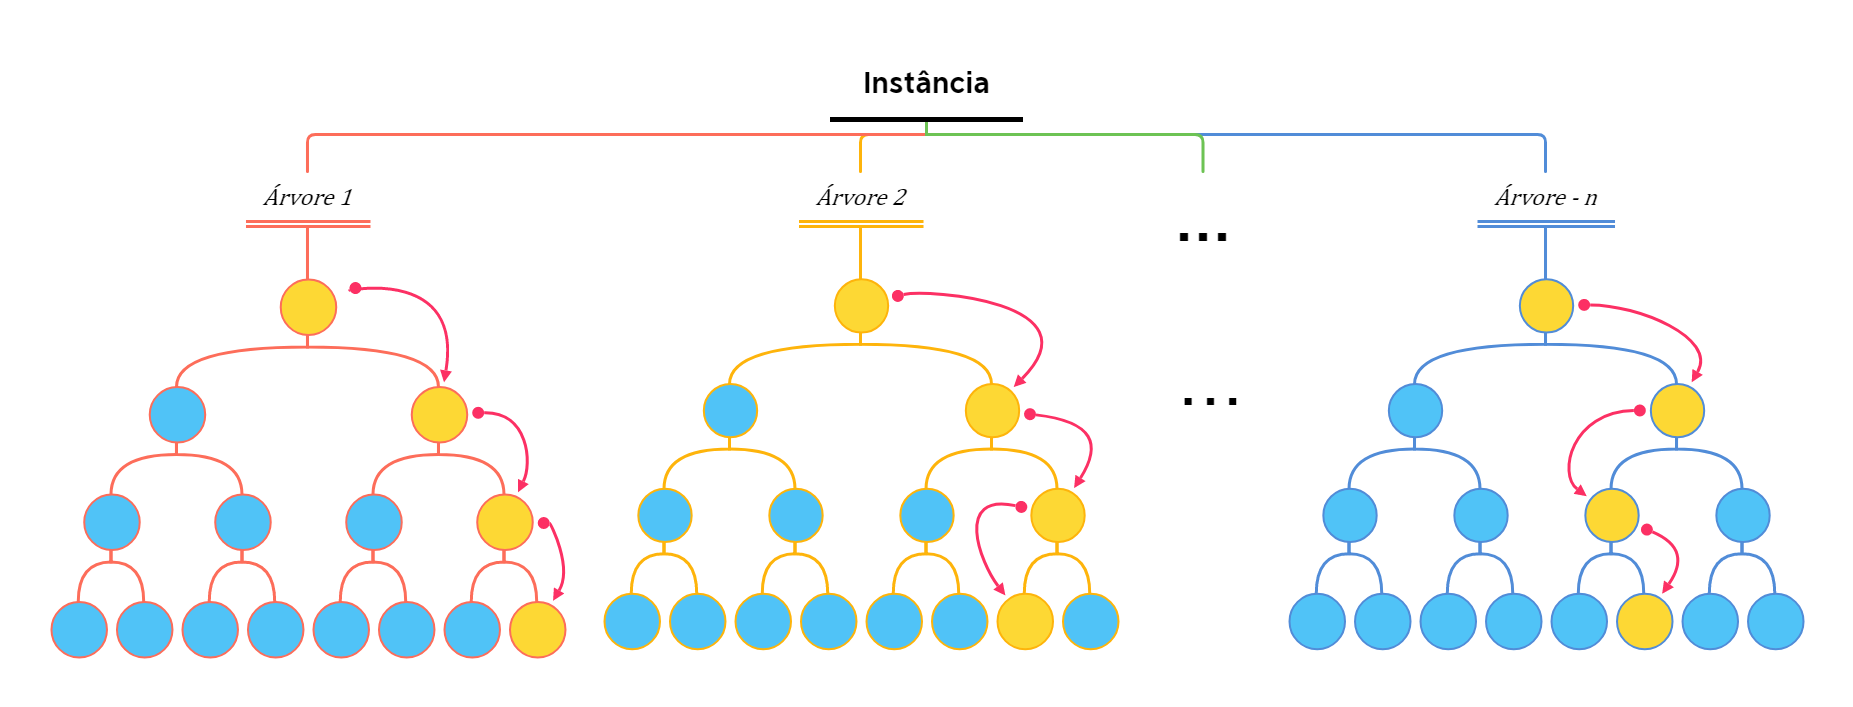
\includegraphics[width=1\linewidth]{Modelos/Figuras/RF}
	
	Fonte: Elaboração própria
\end{figure}


\subsubsection{LightGBM e XGboost}\label{subsubsec:lgbxgb}

O aumento de gradiente combina vários pequenos modelos de árvore de decisão para fazer previsões. É claro que essas pequenas árvores de decisão são diferentes umas das outras, caso contrário não há vantagem em usar mais árvores de decisão. O conceito importante a ser entendido aqui é como essas árvores de decisão se tornam diferentes umas das outras. outros. Isto é conseguido através de um processo chamado elevação. Boosting e bagging são dois métodos principais que são aprendidos juntos.  Boosting é um processo iterativo. Ele adiciona cada vez mais modelos fracos ao conjunto de modelos de maneira inteligente. Em cada etapa, pontos de dados individuais são ponderados.  

Pontos de dados que já estão bem previstos não são importantes para o aluno adicionar. Portanto, novos modelos fracos se concentrarão em aprender coisas que ainda não são compreendidas, melhorando assim o conjunto.

Pode se ver uma visão geral esquemática do processo de reforço na Figura \ref{fig:xgboos}. Com essa abordagem, você ajusta iterativamente modelos fracos que se concentram nas partes dos dados que ainda
não são compreendidas. Ao fazer isso, você mantém todos os modelos fracos intermediários. O modelo ensemble é a combinação de todos esses modelos fracos.


\begin{figure}[H]
	\centering
	\caption{Impulsionando gradiente com XGBoost e LightGBM}
	\label{fig:xgboos}
	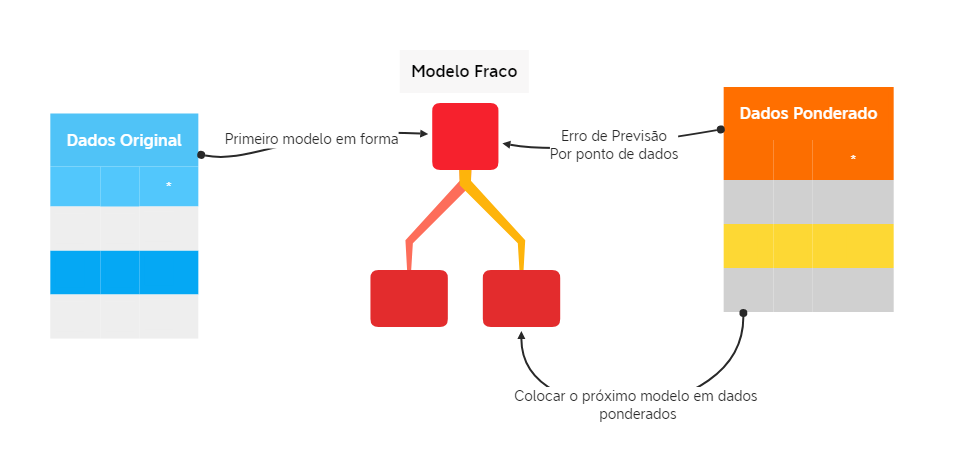
\includegraphics[width=1\linewidth]{Modelos/Figuras/xgboos}
	
	Fonte: Adaptação de \citeonline{korstanje2021}
\end{figure}



\subsubsection{O Gradiente em Gradiente de Boosting (Reforço)} \label{subsubsec:boosting}

\citeonline{korstanje2021} esse processo iterativo é chamado de aumento de gradiente por um motivo. Um gradiente é um termo matemático que se refere ao campo vetorial de derivadas parciais que apontam na direção da inclinação mais acentuada. Em termos simples, muitas vezes comparamos gradientes com declives de estradas em aclive: quanto maior a inclinação, mais íngreme a colina. Os gradientes são calculados tomando derivadas, ou derivadas parciais, de uma função.

No aumento de gradiente, ao adicionar árvores adicionais ao modelo, o objetivo é adicionar uma árvore que melhor explique a variação que não foi explicada pelas árvores anteriores. O destino de sua nova árvore é, portanto.

\begin{eqnarray}
	y-\hat{y}\label{eq:xb}
\end{eqnarray}

De \eqref{eq:xb} isso pode ser denotado reescrito como a derivada parcial negativa da função de perda em relação às previsões de $y$:

\begin{eqnarray}
	y-\hat{y}&=&-\dfrac{\partial L}{\partial \hat{y}}\label{eq:xb2}
\end{eqnarray}

Você define isso como o destino da nova árvore para garantir que a adição da árvore explicará uma quantidade máxima de variação adicional no modelo geral de aumento de gradiente. Isso explica por que o modelo é chamado de aumento de gradiente boosting.

\subsubsection{Algoritmos de boosting de gradiente}

Existem muitos algoritmos que executam versões ligeiramente diferentes de aumento de gradiente. Quando o método de aumento de gradiente foi inventado, o algoritmo não Muito desempenho, mas mudou com o advento do algoritmo AdaBoost: o primeiro algoritmo que pode se adaptar a modelos fracos. 

O algoritmo de aumento de gradiente é uma das ferramentas de aprendizado de máquina com melhor desempenho no mercado. Depois do AdaBoost, uma longa lista de algoritmos de aumento ligeiramente diferentes foi adicionada à literatura, incluindo XGBoost, LightGBM, LPBoost, BrownBoost, MadaBoost, LogitBoost e TotalBoost. Ainda existem muitas contribuições para melhorar a teoria do aumento de gradiente. Nesta subseção, dois algoritmos são apresentados: XGBoost e LightGBM.

O \textbf{XGBoost} é um dos algoritmos de aprendizado de máquina mais usados. O XGBoost é uma maneira rápida de obter bons desempenhos. Como é fácil de usar e tem alto desempenho, é o primeiro algoritmo para muitos profissionais de aprendizado de máquina.

\textbf{LightGBM} é outro algoritmo de aumento de gradiente que é importante conhecer. No momento, é um pouco menos difundido que o XGBoost, mas está ganhando popularidade seriamente.
A vantagem esperada do LightGBM sobre o XGBoost é um ganho de velocidade e uso de memória.
Nesta subseção, você descobrirá as implementações de ambos os algoritmos de aumento de gradiente.

\subsubsection{A diferença entre XGBoost e LightGBM}

Se você for usar esses dois algoritmos de aumento de gradiente, é importante entender de
que maneira eles diferem. Isso também pode fornecer uma visão dos tipos de diferença que fazem um número tão grande de modelos no mercado.

É importante entender se você planeja usar os dois algoritmos de aumento de gradiente
Como eles são diferentes. Isso também fornece informações sobre as várias diferenças que acompanham tantos modelos no mercado.

A diferença aqui é a forma como eles identificam as melhores divisões entre os azarões. (árvores de decisão individuais). Lembre-se de que uma divisão em uma árvore de decisão é quando sua árvore precisa encontrar a divisão que mais melhora seu modelo.

A ideia intuitiva e mais simples para encontrar a melhor divisão é iterar todos os ajustes possíveis e encontrar a melhor divisão. No entanto, isso leva muito tempo e algoritmos recentes apresentam alternativas melhores.
Uma alternativa proposta pelo XGBoost é usar a segmentação baseada em histograma. Nesse caso, ao invés de iterar sobre todas as partições possíveis, o modelo constrói um histograma de cada partição.
variáveis e use-as para encontrar a melhor divisão de variáveis. A melhor divisão geral é então mantida.

LightGBM foi inventado pela Microsoft e tem uma maneira mais eficiente de definir partições. Essa abordagem é chamada de amostragem unilateral baseada em gradiente (GOSS). O GOSS calcula o gradiente de cada ponto de dados e o usa para filtrar pontos de dados com gradientes baixos. Afinal, pontos de dados com gradientes baixos já são bem compreendidos, enquanto indivíduos com gradientes altos precisam ser melhor aprendidos.

O LightGBM também usa uma abordagem chamada Exclusive Feature Bundling (EFB), que permite acelerar a seleção de muitas variáveis correlacionadas. Outra diferença é que o modelo LightGBM é adequado para crescimento de folhas (preferencialmente preferido), enquanto o XGBoost cultiva árvores como árvores. A diferença pode ser vista na Figura \ref{fig:xgboost}.

Essa diferença é um recurso que teoricamente favoreceria o LightGBM em termos de precisão, mas apresenta um risco maior de overfitting (sobreajustamento) no caso de poucos dados disponíveis.

\begin{figure}[H]
	\centering
	\caption{Crescimento em folha versus crescimento em nível}
	\label{fig:xgboost}
	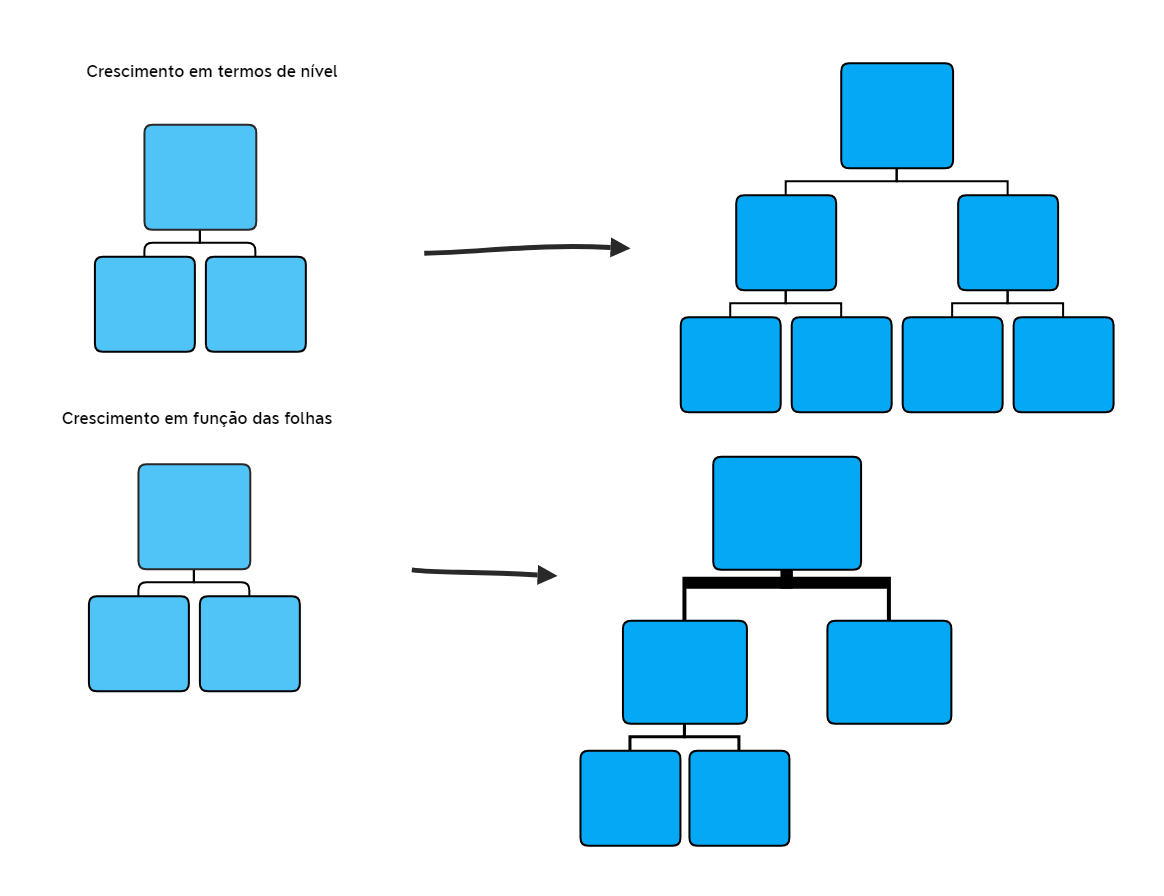
\includegraphics[width=1\linewidth]{Modelos/Figuras/xgboost}
	
	Fonte: Adaptação de \citeonline{korstanje2021}
\end{figure}


Na Figura \ref{fig:xgboost} pode ser visto como cada modelo é ajustado, no crescimento da árvore em folha e em nível.



